%% Version 4.3.2, 25 August 2014
%
%%%%%%%%%%%%%%%%%%%%%%%%%%%%%%%%%%%%%%%%%%%%%%%%%%%%%%%%%%%%%%%%%%%%%%
% Template.tex --  LaTeX-based template for submissions to the 
% American Meteorological Society
%
% Template developed by Amy Hendrickson, 2013, TeXnology Inc., 
% amyh@texnology.com, http://www.texnology.com
% following earlier work by Brian Papa, American Meteorological Society
%
% Email questions to latex@ametsoc.org.
%
%%%%%%%%%%%%%%%%%%%%%%%%%%%%%%%%%%%%%%%%%%%%%%%%%%%%%%%%%%%%%%%%%%%%%
% PREAMBLE
%%%%%%%%%%%%%%%%%%%%%%%%%%%%%%%%%%%%%%%%%%%%%%%%%%%%%%%%%%%%%%%%%%%%%

%% Start with one of the following:
% DOUBLE-SPACED VERSION FOR SUBMISSION TO THE AMS
\documentclass{ametsoc}

% TWO-COLUMN JOURNAL PAGE LAYOUT---FOR AUTHOR USE ONLY
% \documentclass[twocol]{ametsoc}

%%%%%%%%%%%%%%%%%%%%%%%%%%%%%%%%
%%% To be entered only if twocol option is used

\journal{jas}

%  Please choose a journal abbreviation to use above from the following list:
% 
%   jamc     (Journal of Applied Meteorology and Climatology)
%   jtech     (Journal of Atmospheric and Oceanic Technology)
%   jhm      (Journal of Hydrometeorology)
%   jpo     (Journal of Physical Oceanography)
%   jas      (Journal of Atmospheric Sciences)	
%   jcli      (Journal of Climate)
%   mwr      (Monthly Weather Review)
%   wcas      (Weather, Climate, and Society)
%   waf       (Weather and Forecasting)
%   bams (Bulletin of the American Meteorological Society)
%   ei    (Earth Interactions)

%%%%%%%%%%%%%%%%%%%%%%%%%%%%%%%%
%Citations should be of the form ``author year''  not ``author, year''
\bibpunct{(}{)}{;}{a}{}{,}

%%%%%%%%%%%%%%%%%%%%%%%%%%%%%%%%

%%% To be entered by author:

%% May use \\ to break lines in title:

\title{Tropopause Evolution in a Rapidly Intensifying Tropical Cyclone: A Static Stability Budget Analysis}

%%% Enter authors' names, as you see in this example:
%%% Use \correspondingauthor{} and \thanks{Current Affiliation:...}
%%% immediately following the appropriate author.
%%%
%%% Note that the \correspondingauthor{} command is NECESSARY.
%%% The \thanks{} commands are OPTIONAL.

    %\authors{Author One\correspondingauthor{Author One, 
    % American Meteorological Society, 
    % 45 Beacon St., Boston, MA 02108.}
% and Author Two\thanks{Current affiliation: American Meteorological Society, 
    % 45 Beacon St., Boston, MA 02108.}}

\authors{Patrick Duran\correspondingauthor{Department of Atmospheric and Environmental Sciences, University at Albany, State University of New York, 1400 Washington Avenue, Albany, NY.} and John Molinari}

%% Follow this form:
    % \affiliation{American Meteorological Society, 
    % Boston, Massachusetts.}

\affiliation{University at Albany, State University of New York,
Albany, NY}

%% Follow this form:
    %\email{latex@ametsoc.org}

\email{pduran2008@gmail.com}

%% If appropriate, add additional authors, different affiliations:
    %\extraauthor{Extra Author}
    %\extraaffil{Affiliation, City, State/Province, Country}

%\extraauthor{}
%\extraaffil{}

%% May repeat for a additional authors/affiliations:

%\extraauthor{}
%\extraaffil{}

%%%%%%%%%%%%%%%%%%%%%%%%%%%%%%%%%%%%%%%%%%%%%%%%%%%%%%%%%%%%%%%%%%%%%
% ABSTRACT
%
% Enter your abstract here
% Abstracts should not exceed 250 words in length!
%
% For BAMS authors only: If your article requires a Capsule Summary, please place the capsule text at the end of your abstract
% and identify it as the capsule. Example: This is the end of the abstract. (Capsule Summary) This is the capsule summary. 

\abstract{We have some cool results!}

\begin{document}

%% Necessary!
\maketitle


%%%%%%%%%%%%%%%%%%%%%%%%%%%%%%%%%%%%%%%%%%%%%%%%%%%%%%%%%%%%%%%%%%%%%
% MAIN BODY OF PAPER
%%%%%%%%%%%%%%%%%%%%%%%%%%%%%%%%%%%%%%%%%%%%%%%%%%%%%%%%%%%%%%%%%%%%%
%

%% In all cases, if there is only one entry of this type within
%% the higher level heading, use the star form: 
%%
 \section{Introduction}

%Perhaps introduce upper-tropospheric static stability and its relationship to the diurnal cycle before going into Patricia? Include references to Dunion, Navarro, and O'Neill here.
%More recently, \cite{Dunionetal2014} documented a periodic oscillation of infrared brightness temperature in hurricanes, which they call the "TC diurnal pulse."
%There will be a whole bunch of papers cited here...
%At some point (probably in the Discussion) mention the possible importance of static stability asymmetries, in the context of the Dunion diurnal pulse 

After undergoing a remarkably rapid intensification (RI), Hurricane Patricia (2015) set a new record as the strongest tropical cyclone (TC) ever observed in the Western Hemisphere (\citeauthor{Kimberlainetal2016} \citeyear{Kimberlainetal2016}; \citeauthor{Rogersetal2017} \citeyear{Rogersetal2017}).
High-altitude dropsonde observations taken during the Tropical Cyclone Intensity (TCI) experiment captured this RI in unprecedented detail \citep{DoyleTCI}.
These observations revealed remarkable changes in the structure of the cold-point tropopause and upper-level static stability as the storm intensified \citep{DuranMolinari2018}.

At tropical storm intensity, shortly before RI commenced, a strong inversion layer existed just above Patricia's cold-point tropopause, which was located near 17.2 km.
During the first half of the RI period, this inversion layer weakened throughout Patricia's inner core, with the weakening most pronounced over the developing eye.
By the time the storm reached its maximum intensity, the inversion layer over the eye had disappeared almost completely, which was accompanied by an increase in the tropopause height to a level at or above the highest-available dropsonde data point (18.3 km) at two locations.
Meanwhile over the eyewall region, the static stability re-strengthened and the tropopause was limited to a level at or below 17.5 km.
The mechanisms that led to these changes in upper-level static stability and tropopause height are the subject of the current paper.

Despite the importance of tropopause-layer thermodynamics in theoretical models of hurricanes (\citeauthor{EmanuelRotunno2011} \citeyear{EmanuelRotunno2011}; \citeauthor{Emanuel2012} \citeyear{Emanuel2012}), few papers have examined the upper-tropospheric evolution of TCs.
\cite{KomaromiDoyle2017} found that stronger TCs tended to have a higher and warmer tropopause over their inner core than weaker TCs.
Their results are consistent with the evolution observed over the inner core of Hurricane Patricia, in which the tropopause height increased and the tropopause temperature warmed throughout RI \citep{DuranMolinari2018}.
The simulations of \cite{OhnoSatoh2015} suggested that the development of an upper-level warm core within the eye acted to decrease the static stability near the tropopause.
Although the mechanisms that drive this static stability evolution have not been examined explicitly, the potential temperature ($\theta$) budget analysis of \cite{SternZhang2013} examined the development of the TC warm core.
They found that radial and vertical advection both play important roles in warm core development throughout RI, with subgrid-scale diffusion becoming particularly important during the later stage of RI.

The analysis herein is based upon that of \cite{SternZhang2013}, except using a static stability budget similar to that of \cite{Kepertetal2016} rather than a $\theta$ budget.

 \section{Model Setup}

The numerical simulations were performed using version 19.4 of Cloud Model 1 (CM1) described in \cite{BryanRotunno2009}.
The equations of motion were integrated on a 3000-km-wide, 30-km-deep axisymmetric grid with 1-km horizontal and 250-m vertical grid spacing.
The computations were performed on an \textit{f}-plane at 15\textdegree{N} latitude, over a sea surface with constant temperature of 30.5\textdegree C, which matches that observed near Hurricane Patricia (2015; \citeauthor{Kimberlainetal2016} \citeyear{Kimberlainetal2016}).
Horizontal turbulence was parameterized using the Smagorinsky scheme described in \citeauthor{BryanRotunno2009} (\citeyear{BryanRotunno2009}, pg. 1773), with a prescribed mixing length that varied linearly from 100 m at a surface pressure of 1015 hPa to 1000 m at a surface pressure of 900 hPa.
This formulation allows for realistically-large horizontal mixing lengths near the hurricane's inner core, consistent with the results of \cite{Bryan2012}, while not over-representing horizontal turbulence in convection at outer radii.
Vertical turbulence was parameterized using the formulation of \citeauthor{MarkowskiBryan2016} (\citeyear{MarkowskiBryan2016}, their Eq. 6), using an asymptotic vertical mixing length of 100 m.
A Rayleigh damping layer was applied outside of the 2900-km radius and above the 25-km level to prevent spurious gravity wave reflection at the model boundaries.
Microphysical processes were parameterized using the \cite{Thompson} microphysics scheme and radiative heating tendencies were computed every two minutes using the Rapid Radiative Transfer Model for GCMs (RRTMG) longwave and shortwave schemes \citep{Iacono}.
The initial temperature and humidity field was horizontally homogeneous and determined by averaging all Climate Forecast System Reanalysis (CFSR) grid points within 100 km of Patricia's center of circulation at 18 UTC 21 October 2015.
%A horizontally-homogeneous temperature and humidity field was initialized with a mean sounding computed using all dropsondes deployed during the TCI flight conducted within and around Tropical Storm Patricia on 21 October, 2015 (see \citeauthor{DoyleTCI} \citeyear{DoyleTCI} for details.)
%Above 19 km, where few TCI observations were available, the temperature profile was taken from the Climate Forecast System Reanalysis (CFSR) grid point nearest Patricia's storm center, valid at 18 UTC 21 October, 2015.
%Since relative humidity measurements were unreliable at temperatures below -40\textdegree C \citep{BellTCI}, relative humidity was set equal to 50\% above 11.5 km (the level above which temperature dropped below -40\textdegree C).
The vortex described in \citeauthor{RotunnoEmanuel} (\citeyear{RotunnoEmanuel}, their Eq. 37) was used to initialize the wind field, setting all parameters equal to the values used therein.

Although hurricanes simulated in an axisymmetric framework tend to be more intense than those observed in nature, the intensity evolution of this simulation matches reasonably well with that observed in Hurricane Patricia.
After an initial spin-up period of about 20 hours, the modeled storm (Fig.\ref{fig:vmax+pmin}, blue lines) began an RI period that lasted approximately 30 hours.
After this RI, the storm continued to intensify more slowly until the maximum 10-m wind speed reached 89 m s\textsuperscript{-1} and the minimum sea-level pressure reached its minimum of 846 mb, 81 hours into the simulation.
Hurricane Patricia (red stars) exhibited a similar intensity evolution, with an RI period leading to a maximum 10-m wind speed of 95 m s\textsuperscript{-1} and a minimum sea-level pressure of 872 hPa.
Despite the limitations of the axisymmetric framework, the extraordinary intensity of Hurricane Patricia and the rapidity of its intensification makes Patricia a particularly good candidate for axisymmetric analysis.

 \section{Budget Computation}

The static stability can be expressed as the squared Brunt V{\"a}is{\"a}l{\"a} frequency:
   \begin{equation} \label{eq:n2moist}
   N_m^2 = \frac{g}{T}\left(\frac{\partial T}{\partial z}+\Gamma_m\right)\left(1+\frac{T}{R_d/R_v+q_s}\frac{\partial q_s}{\partial T}\right)-\frac{g}{1+q_t}\frac{\partial q_t}{\partial z},
   \end{equation}
where $g$ is gravitational acceleration, $T$ is temperature, $R_d$ and $R_v$ are the gas constants of dry air and water vapor, respectively, $q_s$ is the saturation mixing ratio, $q_t$ is the total condensate mixing ratio, and $\Gamma_m$ is the moist-adiabatic lapse rate:
   \begin{equation} \label{eq:gamma_m}
   \Gamma_m = g(1+q_t)\left(\frac{1+L_vq_s/R_dT}{c_p_m +L_v\partial q_s/\partial T}\right),
   \end {equation}
where $L_v$ is the latent heat of vaporization and $c_{pm}$ is the specific heat of moist air at constant pressure.
In the tropopause layer, $q_s$, ${\partial q_s}/{\partial T}$, and ${\partial q_t}/{\partial z}$ approach zero. In this limiting case, Eq. \ref{eq:n2moist} reduces to:
   \begin{equation} \label{eq:n2dry}
   N^2 = \frac{g}{\theta_v}\frac{\partial \theta_v}{\partial z},
   \end{equation}
where $\theta_v$ is the virtual potential temperature.
To compute $N^2$, CM1 uses Eq.\ref{eq:n2moist} in saturated environments and Eq. \ref{eq:n2dry} in sub-saturated environments. For simplicity, however, only Eq. \ref{eq:n2dry} will be employed for the budget computations herein\footnote{The validity of this approximation will be substantiated later in this section.}.

Taking the time derivative of Eq. \ref{eq:n2dry} yields the static stability tendency:
   \begin{equation} \label{eq:dn2dt}
   \frac{\partial N^2}{\partial t} = \frac{g}{\theta}\frac{\partial}{\partial z}\frac{\partial \theta}{\partial t}-\frac{g}{\theta^2}\frac{\partial \theta}{\partial z}\frac{\partial \theta}{\partial t},
   \end{equation}
where the potential temperature tendency, $\partial \theta/\partial t$, can be written:
   \begin{equation} \label{eq:dthetadt}
   \frac{\partial \theta}{\partial t} = HADV+VADV+HTURB+VTURB+MP+RAD+DISS 
   \end{equation}
Each term on the right-hand side of Eq. \ref{eq:dthetadt} represents a $\theta$ budget variable, each of which is output directly by the model every minute.
HADV and VADV are the radial and vertical advective tendencies, HTURB and VTURB are the radial and vertical tendencies from the turbulence parameterization, MP is the tendency from the microphysics scheme, RAD is the tendency from the radiation scheme, and DISS is the tendency due to turbulent dissipation.
This equation neglects Rayleigh damping, since this term is zero everywhere below 25 km, and the analysis domain does not extend to that level.
Each term in Eq. \ref{eq:dthetadt} is substituted for ${\partial \theta}/{\partial t}$ in Eq. \ref{eq:dn2dt}, yielding the contribution of each budget term to the static stability tendency.
These terms are summed, yielding an instantaneous "budget change" in $N^2$ every minute.
The budget changes are then averaged over 24-hour periods and compared to the total model change in $N^2$ over that same time period, i.e.:
   \begin{equation} \label{eq:budgetchange}
   \Delta N^2_{budget} = \frac{1}{\delta t}\sum_{t=t_0}^{t_0+\delta t} \left.\frac{\partial N^2}{\partial t}\right\vert_t
   \end{equation}
   \begin{equation} \label{eq:modelchange}
   \Delta N^2_{model} = N^2_{t_0+\delta t}-N^2_{t_0}
   \end{equation}
   \begin{equation} \label{eq:residual}
   Residual = \Delta N^2_{model}-\Delta N^2_{budget}
   \end{equation}
where $t_0$ is an initial time and $\delta t$ is 24 hours.

Eqs. \ref{eq:budgetchange}-\ref{eq:residual} are plotted for four consecutive 24-hour periods in Fig. \ref{fig:mod+bud+res}.
For this and all subsequent radial-vertical cross sections, a 1-2-1 smoother is applied once in the radial direction to eliminate $2\Delta r$ noise that appears in some of the raw model output and calculated fields.
The left column of Fig.~\ref{fig:mod+bud+res} depicts the model changes (Eq. \ref{eq:modelchange}), the center column depicts the budget changes (Eq. \ref{eq:budgetchange}), and the right column depicts the residuals (Eq. \ref{eq:residual}).
In every 24-hour period, the budget changes are nearly identical to the model changes, which is reflected in the near-zero residuals in the right column.
This indicates that the budget accurately represents the model variability, which implies that the neglect of moisture in the budget computation introduces negligible error within the anaysis domain\footnote{This is not the case in the lower- and mid-troposphere, where the residual actually exceeds the budget variability in many places, likely due to the neglect of moisture; thus we limit this analysis to the upper troposphere and lower stratosphere.}.

In the tropopause layer, some of the budget terms are small enough to be ignored.
To determine which of the budget terms are most important, a time series of the contribution of each of the budget terms in Eq. \ref{eq:dthetadt} to the tropopause-layer static stability tendency is plotted in Fig. \ref{fig:avgbudterms}.
For this figure, each of the budget terms is computed using the method described in Section 3, except with 1-hour averaging intervals instead of 24-hour intervals.
The absolute values of these tendencies are then averaged over a radius-height domain surrounding the tropopause and plotted as a time series\footnote{It will be seeen in subsequent figures that each of the terms contributes both positively and negatively to the N\textsuperscript{2} tendency within the analysis domain. 
Thus, taking an average over the domain tends to wash out the positive and negative contributions.
To circumvent this problem, the absolute value of each of the terms is averaged.}. 
Advection (Fig.~\ref{fig:avgbudterms}, red line) plays an important role in the mean tropopause-layer static stability tendency at all times, and vertical turbulence (Fig.~\ref{fig:avgbudterms}, blue line) and radiation (Fig.~\ref{fig:avgbudterms}, dark green line) also contribute significantly. %both become important after 48 hours.
Although the contribution from horizontal turbulence (Fig.~\ref{fig:avgbudterms}, purple line) becomes more important after 48 hours, it is confined to a very small region immediately surrounding the eyewall tangential velocity maximum (not shown), and is negligible throughout the rest of the tropopause layer.
The remaining two processes - microphysics and dissipative heating (Fig.~\ref{fig:avgbudterms}, orange and light green lines, respectively) - lie atop one another near zero.
These time series indicate that, at all times, three budget terms dominate the tropopause-layer static stability tendency: advection, vertical turbulence, and radiation.
Variations in the magnitude and spatial structure of these terms drive the static stability changes depicted in Fig.~\ref{fig:mod+bud+res}; subsequent sections will focus on these variations and what causes them.

 \section{Results}

 \subsection{Static stability evolution}

The average $N^2$ over the first day of the simulation (Fig.~\ref{fig:n2-24hr-avgs}a) indicates the presence of a weak static stability maximum just above the cold-point tropopause.
Over the subsequent 24 hours, during which RI occurred, this static stability maximum weakened within the 20 km radius (Fig.~\ref{fig:n2-24-hr-avgs}b).
This decreasing $N^2$ corresponded to an increase in the tropopause height within the developing eye, maximizing at the storm center.
Outside of the eye, meanwhile, the tropopause height decresed over the eyewall region (25-60-km radius) and increased only slightly outside of the 60 km radius.
In this outer region, the lower-stratospheric $N^2$ maximum strengthened during RI.
These trends continued as the storm's intensity leveled off in the 48-72-hour period (Fig.~\ref{fig:n2-24hr-avgs}c).
The tropopause height increased to nearly 21 km at the storm center and sloped sharply downward to 16.3 km on the inner edge of the eyewall, near the 30 km radius.
This static stability evolution closely follows that observed in Hurricane Patricia (2015; \citeauthor{DuranMolinari2018} \citeyear{DuranMolinari2018}).
Since most of the static stability variability 

 \subsection{Static stability budget analysis}

\paragraph{0-24 hours}
The first 24 hours of the simulation was characterized by a weakening of the lower-stratospheric static stability maximum above 17 km (Fig.~\ref{fig:stab-0-24}a, purple shading) and an increase in static stability below (green shading).
Although these tendencies extended out to the 200-km radius, they were particularly pronounced at innermost radii.
A comparison of the contributions of advection (Fig.~\ref{fig:stab-0-24}b), vertical turbulence (Fig.~\ref{fig:stab-0-24}c), and radiation (Fig.~\ref{fig:stab-0-24}d) reveals that advection is primarily responsible for the change in static stability during this period.
...Explain this in the context of radial and vertical velocities...

\paragraph{24-48 hours}
During the second day of the simulation, the lower-stratospheric stable layer continued to weaken (Fig.~\ref{fig:stab-24-48}a).
This weakening trend in the 16.75-17.75-km layer extended from the 50 km radius outward to past 200 km, and was primarily driven by advection (Fig.~\ref{fig:stab-24-48}b).
Below this layer, static stability began to increse slightly.
This stabilization had contributions from both vertical turbulence (Fig.~\ref{fig:stab-24-48}c) and radiation (Fig.~\ref{fig:stab-24-48}d) in the 16-16.5-km layer.
...Explain this in context of mean vertical mixing coefficient and mean radiative heating tendency...
Meanwhile, radially inward of 60 km, static stability below 17.5 km continued to weaken, primarily due to advective processes.

\paragraph{48-72 hours}
The third day of the simulation marked a dramatic change in the structure of the tropopause-layer static stability tendencies. During this time, static stability increased markedly in an upward-sloping region within the 30-60-km radial band (Fig.~\ref{fig:stab-48-72}a), and also increased within the 16.75-17.5-km layer out to at least the 200-km radius.
As this layer stabilized, the layer immediately below it destabilized in a broad region extending from 60-200 km.
Examination of the contribution from total advection (Fig.~\ref{fig:stab-48-72}b) reveals that advection no longer dominates the static stability tendencies.
Instead, a combination of vertical turbulence (Fig.~\ref{fig:stab-48-72}c) and radiation (Fig.~\ref{fig:stab-48-72}d) overcomes the destabilizing influence of advection to create the layer of increasing static stability.
Meanwhile, the destabilizing influence of vertical turbulence in a broad region below 17 km combines with a small region of destabilization due to radiation in the 50-120-km radial band combine to destabilize the layer below 16.5 km in the 50-200-km radial band.
Comparing the sum of advection and vertical turbulence (Fig.~\ref{fig:stab-48-72}e) to the sum of advection, vertical turbulence, and radiation (Fig.~\ref{fig:stab-48-72}f) reveals that radiation plays a fundamental role in the re-strengthening of the lower-stratospheric stable layer during this time.

\paragraph{72-96 hours}

  \section{Discussion}

Radiative heating and turbulence viscosity figures?

Discuss how turbulence increases the static stability in some regions --> vertical gradients of turblence intensity.

Dunion et al. speculate that the diurnal pulse only occurs in mature storms. Maybe the development of the near-tropopause stable layer could partially explain the reason for this.
% text...
% \section{Section title}

%vs

% \section{Section title}
% \subsection{subsection one}
% text...
% \subsection{subsection two}
% \section{Section title}

%%%
% \section{First primary heading}

% \subsection{First secondary heading}

% \subsubsection{First tertiary heading}

% \paragraph{First quaternary heading}

%%%%%%%%%%%%%%%%%%%%%%%%%%%%%%%%%%%%%%%%%%%%%%%%%%%%%%%%%%%%%%%%%%%%%
% ACKNOWLEDGMENTS
%%%%%%%%%%%%%%%%%%%%%%%%%%%%%%%%%%%%%%%%%%%%%%%%%%%%%%%%%%%%%%%%%%%%%
%
\acknowledgments
We are indebted to George Bryan for his continued development and support of Cloud Model 1.
We also thank Jeffrey Kepert, Robert Fovell, and Erika Navarro for helpful conversations related to this work.
ADD GRANT NUMBER

%%%%%%%%%%%%%%%%%%%%%%%%%%%%%%%%%%%%%%%%%%%%%%%%%%%%%%%%%%%%%%%%%%%%%
% APPENDIXES
%%%%%%%%%%%%%%%%%%%%%%%%%%%%%%%%%%%%%%%%%%%%%%%%%%%%%%%%%%%%%%%%%%%%%
%
% Use \appendix if there is only one appendix.
%\appendix

% Use \appendix[A], \appendix}[B], if you have multiple appendixes.
%\appendix[A]

%% Appendix title is necessary! For appendix title:
%\appendixtitle{}

%%% Appendix section numbering (note, skip \section and begin with \subsection)
% \subsection{First primary heading}

% \subsubsection{First secondary heading}

% \paragraph{First tertiary heading}

%% Important!
%\appendcaption{<appendix letter and number>}{<caption>} 
%must be used for figures and tables in appendixes, e.g.,
%

%
% All appendix figures/tables should be placed in order AFTER the main figures/tables, i.e., tables, appendix tables, figures, appendix figures.
%
%%%%%%%%%%%%%%%%%%%%%%%%%%%%%%%%%%%%%%%%%%%%%%%%%%%%%%%%%%%%%%%%%%%%%
% REFERENCES
%%%%%%%%%%%%%%%%%%%%%%%%%%%%%%%%%%%%%%%%%%%%%%%%%%%%%%%%%%%%%%%%%%%%%
% Make your BibTeX bibliography by using these commands:
 \bibliographystyle{ametsoc2014}
 \bibliography{references}

%%%%%%%%%%%%%%%%%%%%%%%%%%%%%%%%%%%%%%%%%%%%%%%%%%%%%%%%%%%%%%%%%%%%%
% TABLES
%%%%%%%%%%%%%%%%%%%%%%%%%%%%%%%%%%%%%%%%%%%%%%%%%%%%%%%%%%%%%%%%%%%%%
%% Enter tables at the end of the document, before figures.
%%
%
%\begin{table}[t]
%\caption{This is a sample table caption and table layout.  Enter as many tables as
%  necessary at the end of your manuscript. Table from Lorenz (1963).}\label{t1}
%\begin{center}
%\begin{tabular}{ccccrrcrc}
%\hline\hline
%$N$ & $X$ & $Y$ & $Z$\\
%\hline
% 0000 & 0000 & 0010 & 0000 \\
% 0005 & 0004 & 0012 & 0000 \\
% 0010 & 0009 & 0020 & 0000 \\
% 0015 & 0016 & 0036 & 0002 \\
% 0020 & 0030 & 0066 & 0007 \\
% 0025 & 0054 & 0115 & 0024 \\
%\hline
%\end{tabular}
%\end{center}
%\end{table}

%%%%%%%%%%%%%%%%%%%%%%%%%%%%%%%%%%%%%%%%%%%%%%%%%%%%%%%%%%%%%%%%%%%%%
% FIGURES
%%%%%%%%%%%%%%%%%%%%%%%%%%%%%%%%%%%%%%%%%%%%%%%%%%%%%%%%%%%%%%%%%%%%%
%% Enter figures at the end of the document, after tables.
%%
%


%FIGURE 1%
\begin{figure}[ht]
\centerline{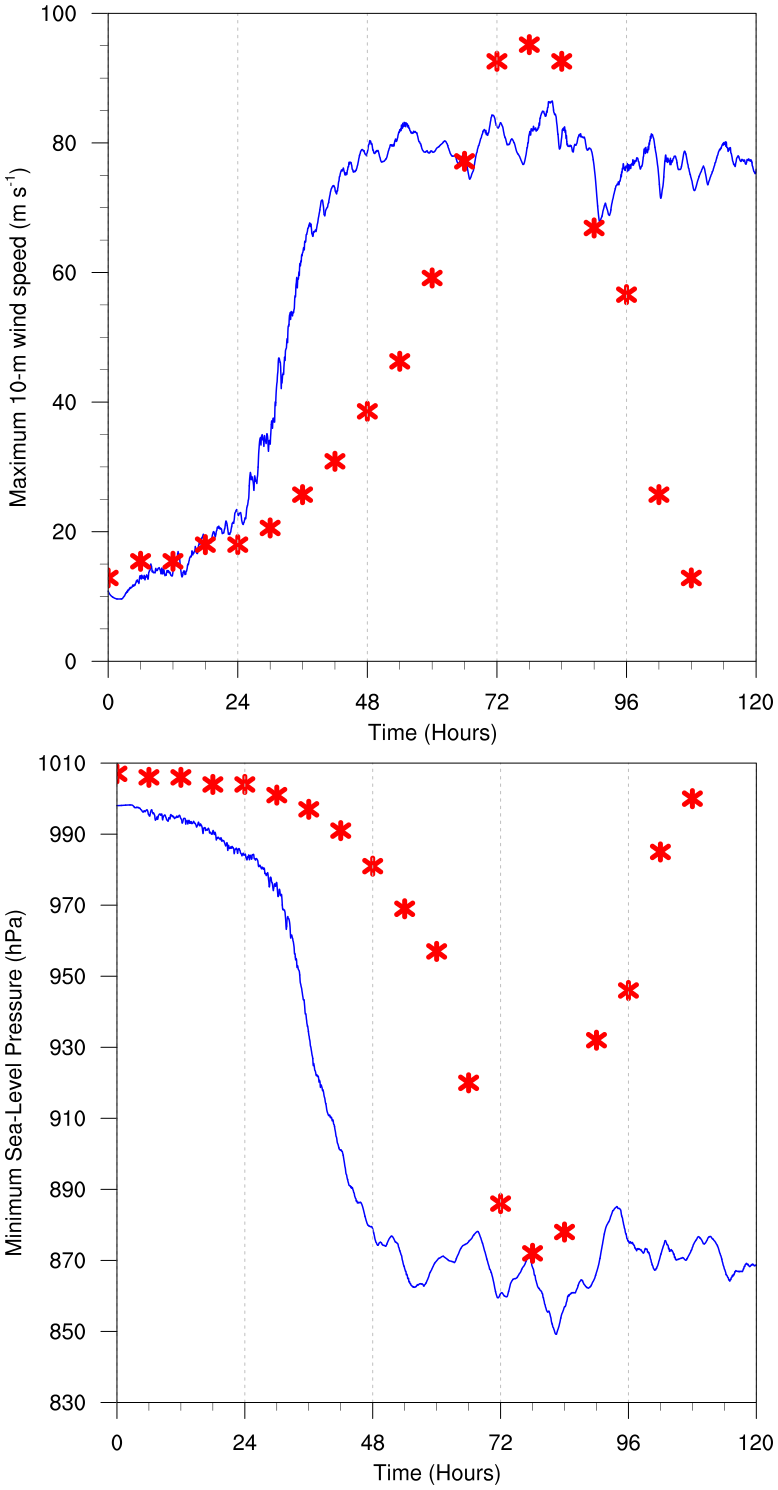
\includegraphics[width=19pc]{figures/vmax+pmin.png}}
\caption{The maximum 10-m wind speed (top panel; m s\textsuperscript{-1}) and minimum sea-level pressure (bottom panel; hPa) in the simulated storm (blue lines) and from Hurricane Patricia's best track (red stars).}
\label{fig:vmax+pmin}
\end{figure}

%FIGURE 2%
\begin{figure}[ht]
\centerline{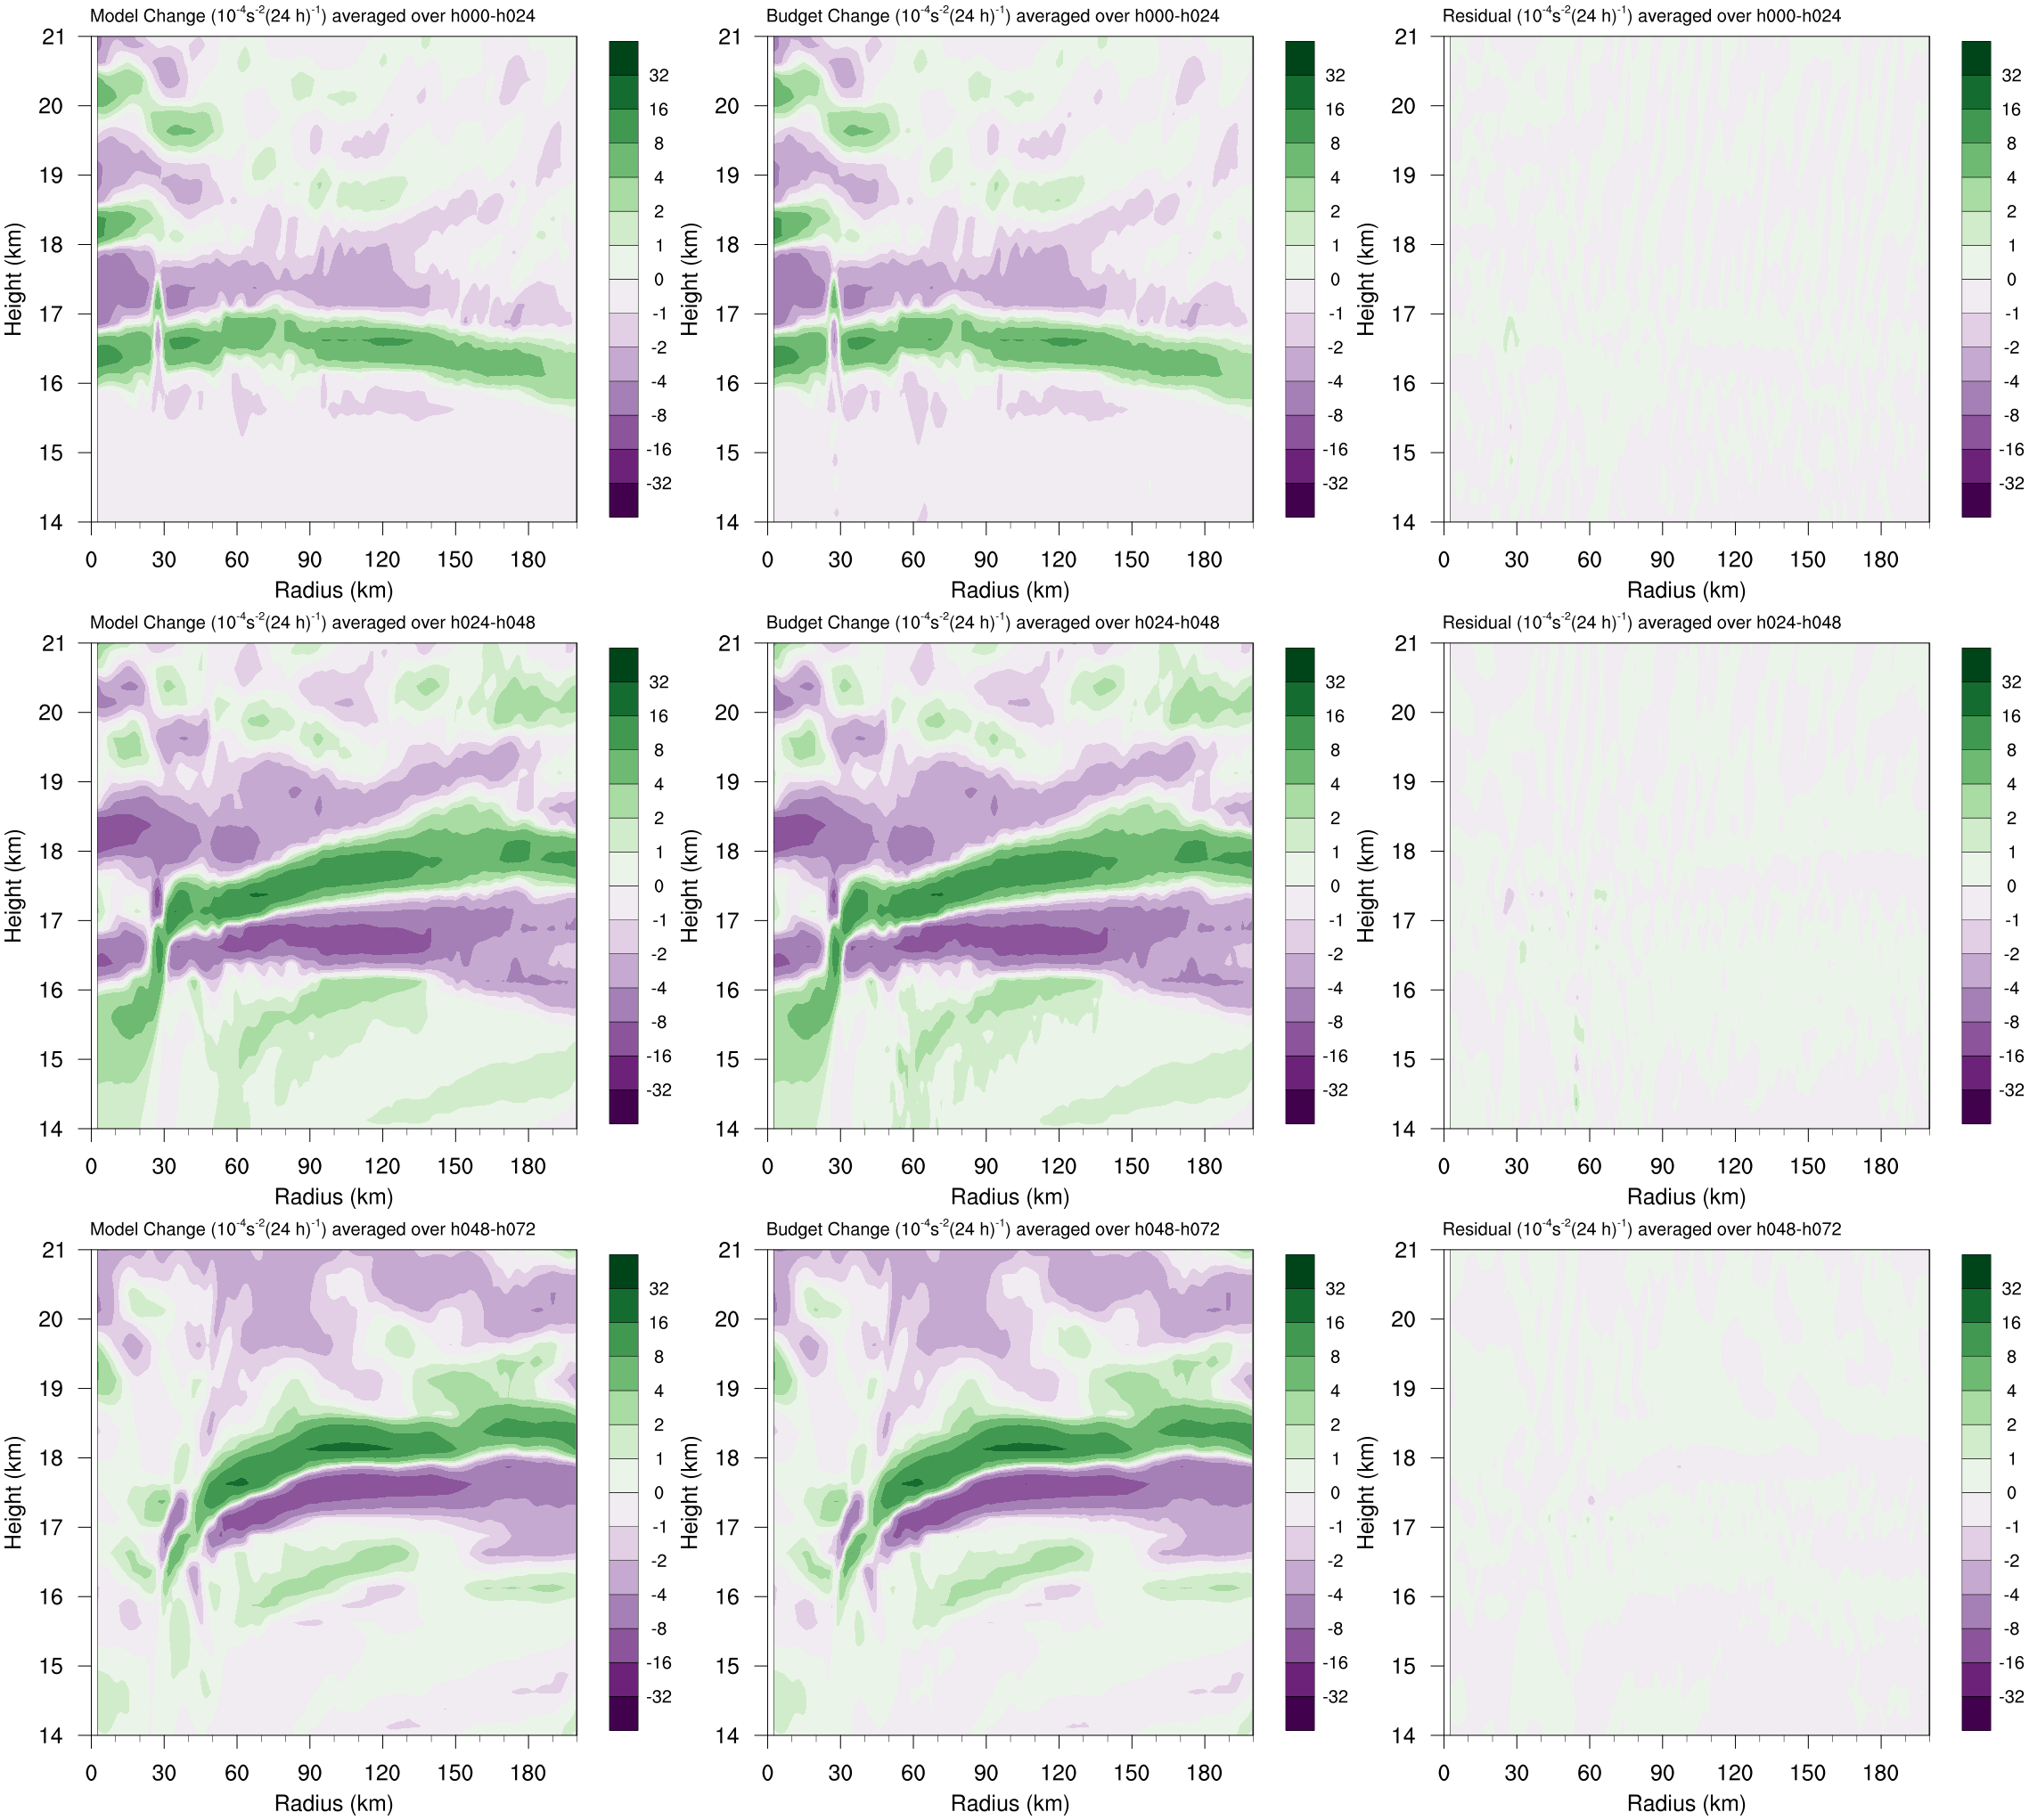
\includegraphics[width=39pc]{figures/mod+bud+res.png}}
\caption{Left panels: Twenty-four-hour changes in squared Brunt-V{\"a}is{\"a}l{\"a} frequency ($N^2$; 10\textsuperscript{-4} s\textsuperscript{-2}) over (a) 0-24 hours, (b) 24-48 hours, (c) 48-72 hours, (d) 72-96 hours. Middle Panels: The $N^2$ change over the same time periods computed using Eq. \ref{eq:budgetchange}. Right Panels: The budget residual over the same time periods, computed by subtracting the budget change (middle column) from the model change (left column).}
\label{fig:mod+bud+res}
\end{figure}

%FIGURE 3%
\begin{figure*}[ht]
\centerline{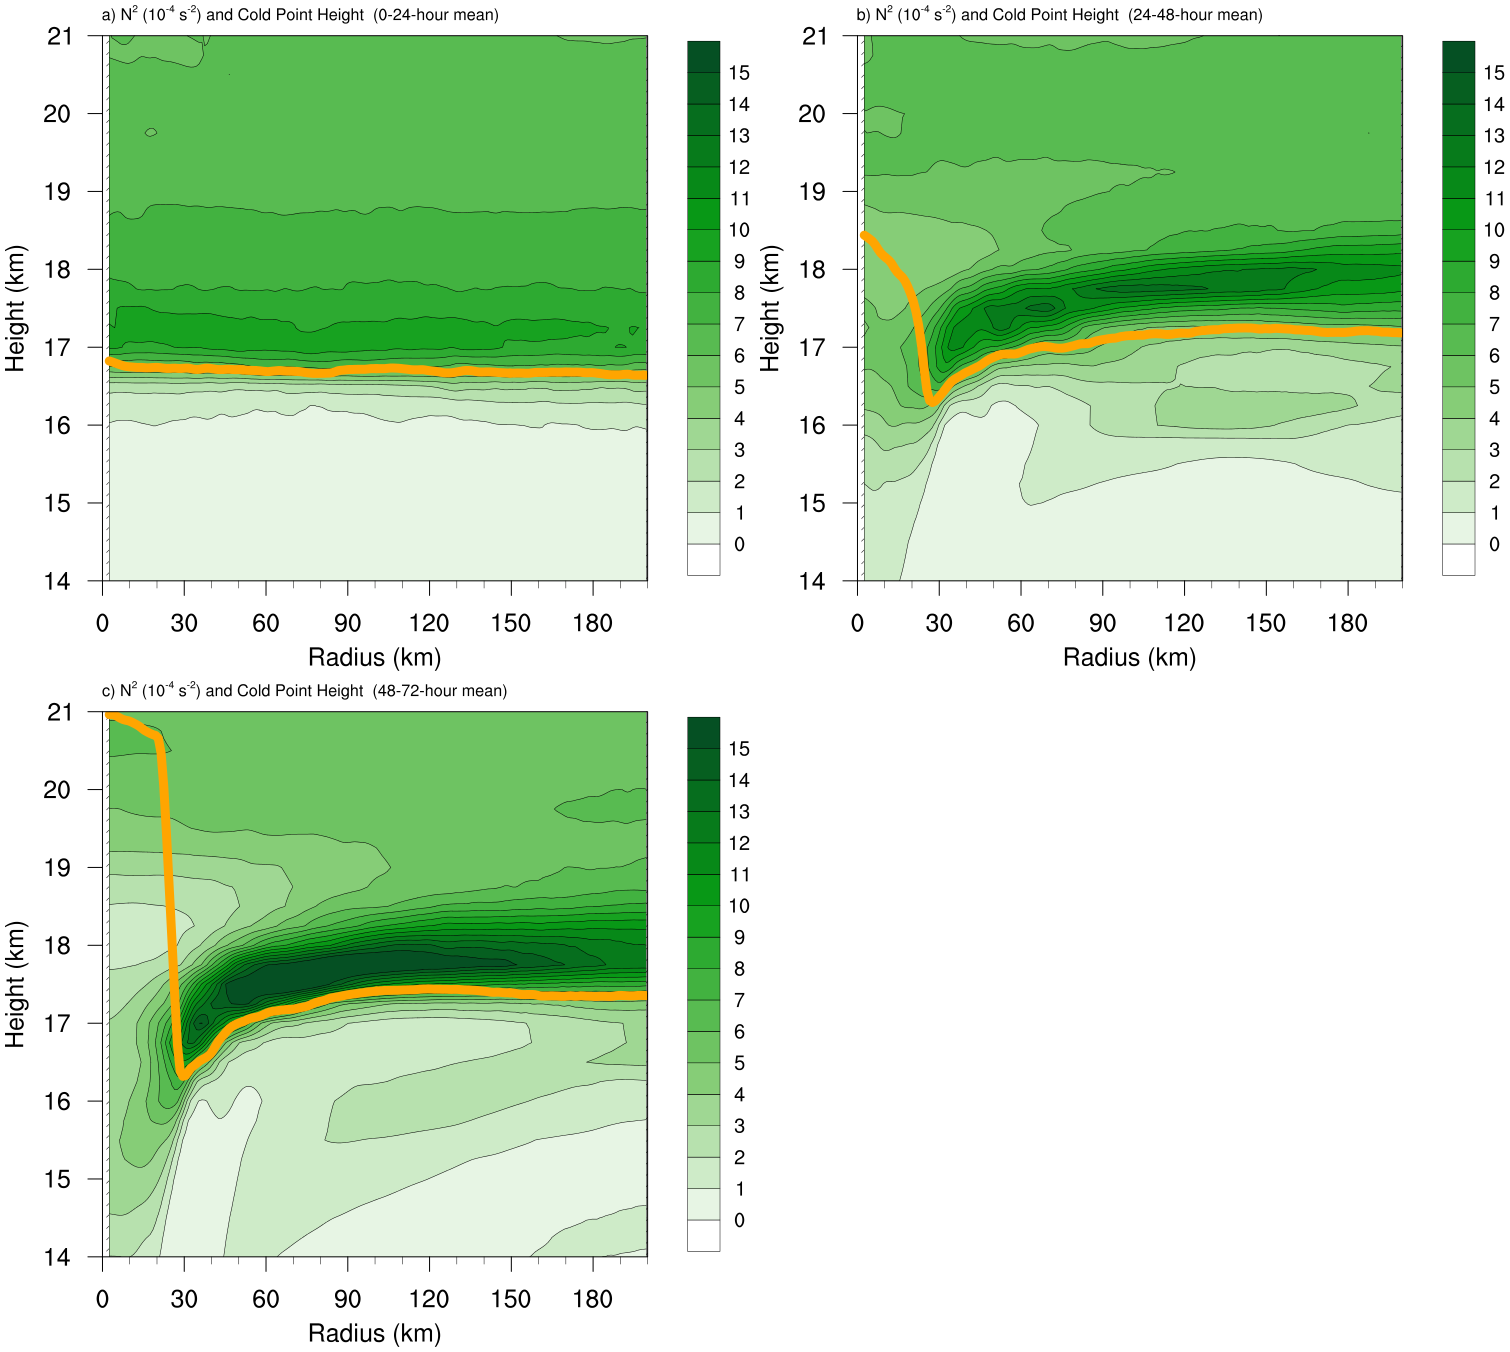
\includegraphics[width=39pc]{figures/n2-24hr-avgs.png}}
\caption{Twenty-four-hour averages of squared Brunt-V{\"a}is{\"a}l{\"a} frequency (10\textsuperscript{-4} s\textsuperscript{-2}) over the first four days of the simulation. Orange lines represent the cold-point tropopause determined by the mean temperature field over the same time periods.}
\label{fig:n2-24hr-avgs}
\end{figure*}

%FIGURE 4%
\begin{figure}[ht]
\centerline{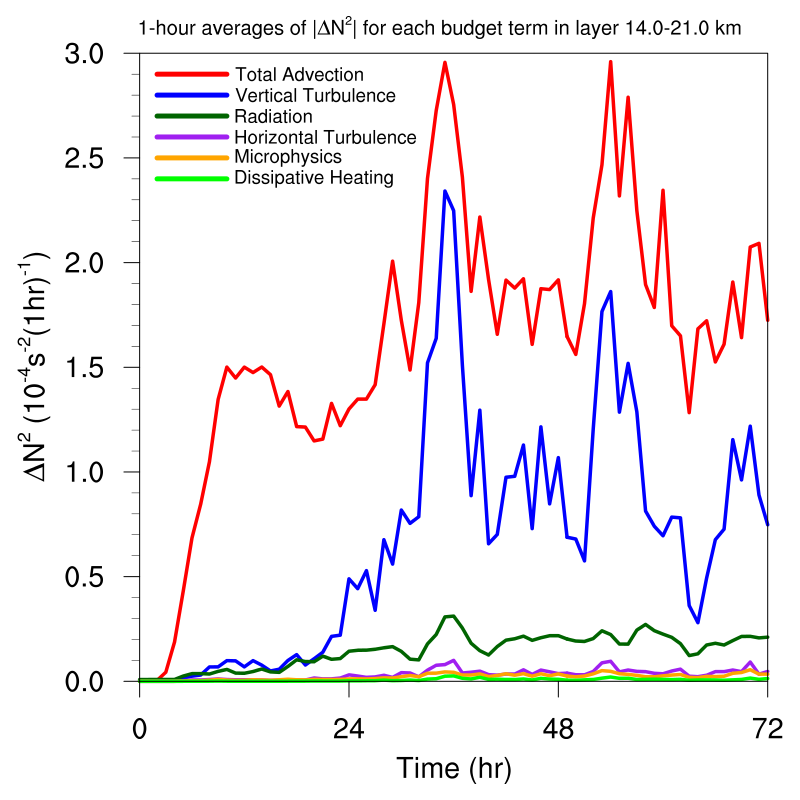
\includegraphics[width=19pc]{figures/AVG_budterms.png}}
\caption{Time series of the contribution of each of the budget terms to the time tendency of the squared Brunt-V{\"a}is{\"a}l{\"a} frequency (N\textsuperscript{2}; 10\textsuperscript{-4} s\textsuperscript{-2}). For each budget term, the absolute value of the N\textsuperscript{2} tendency is averaged temporally over 1-hour periods (using output every minute), and spatially in a region extending from 0 to 200 km radius and 14 to 21 km altitude.}
\label{fig:avgbudterms}
\end{figure}

%FIGURE 5%
\begin{figure*}[ht]
\centerline{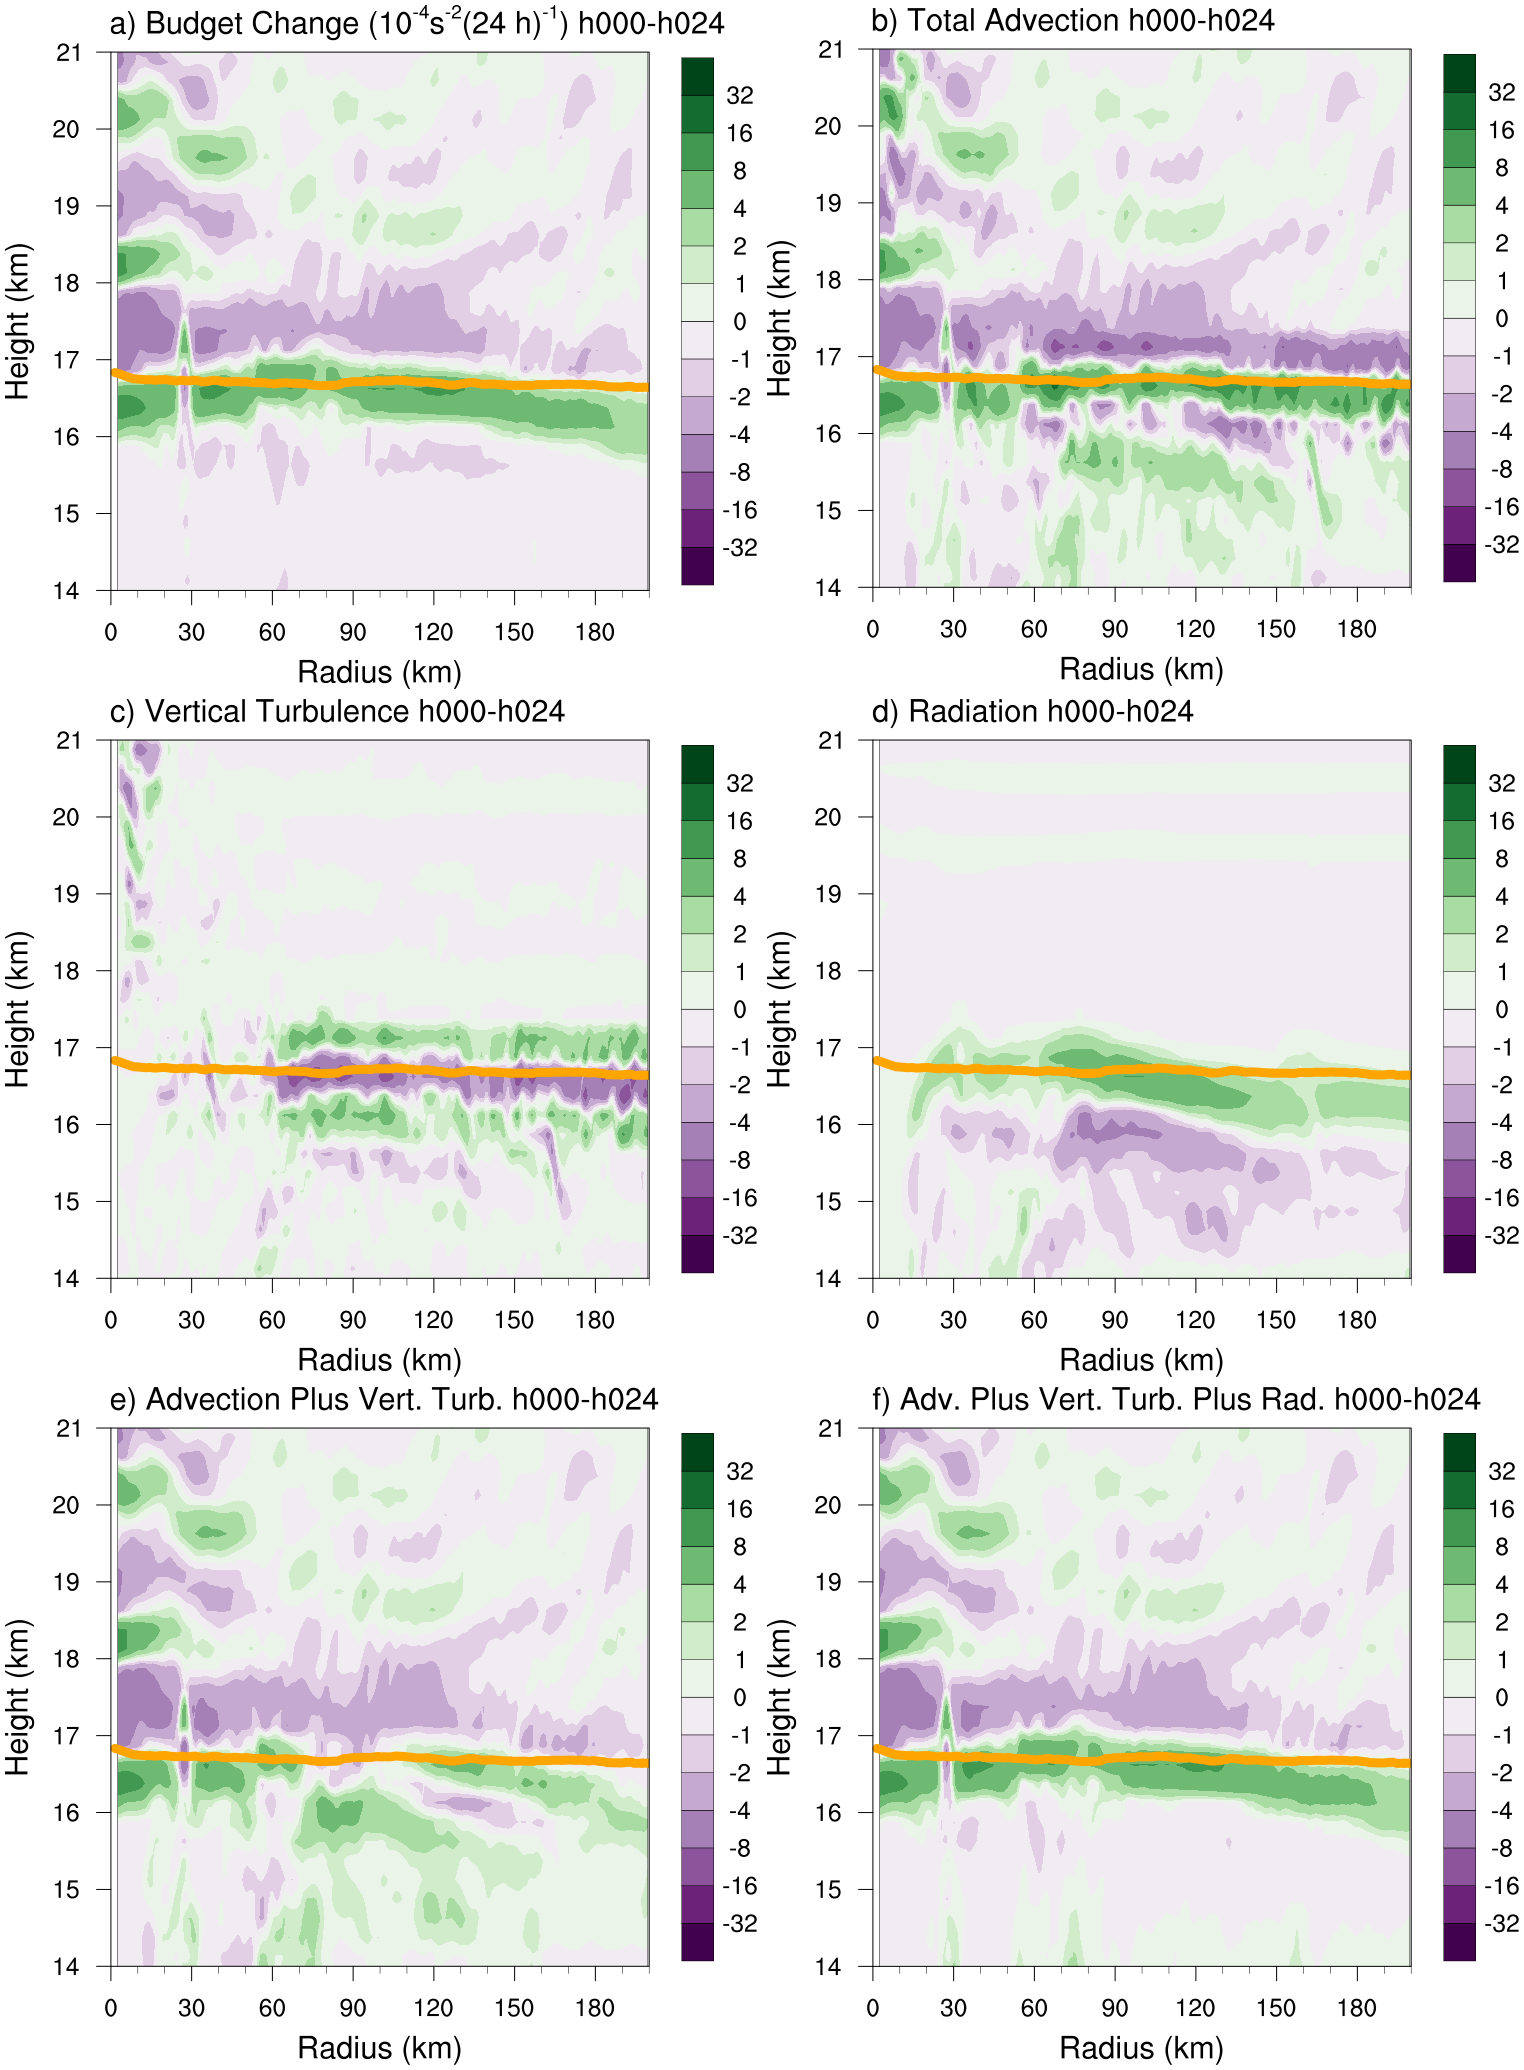
\includegraphics[width=27pc]{figures/h000-h024-budgetterms.png}}
\caption{(a) Total change in N\textsuperscript{2} over the 0-24-hour period (10\textsuperscript{-4} s\textsuperscript{-2} (24 hr)\textsuperscript{-1}) and the contributions to that change from (b) the sum of horizontal and vertical advection, (c) vertical turbulence, (d) longwave and shortwave radiation, (e) the sum of horizontal advection, vertical advection, and vertical turublence, and (f) the sum of horizontal advection, vertical advection, vertical turbulence, and longwave and shortwave radiation.}
\label{fig:stab-00-24}
\end{figure*}

%FIGURE 6%
\begin{figure*}[ht]
\centerline{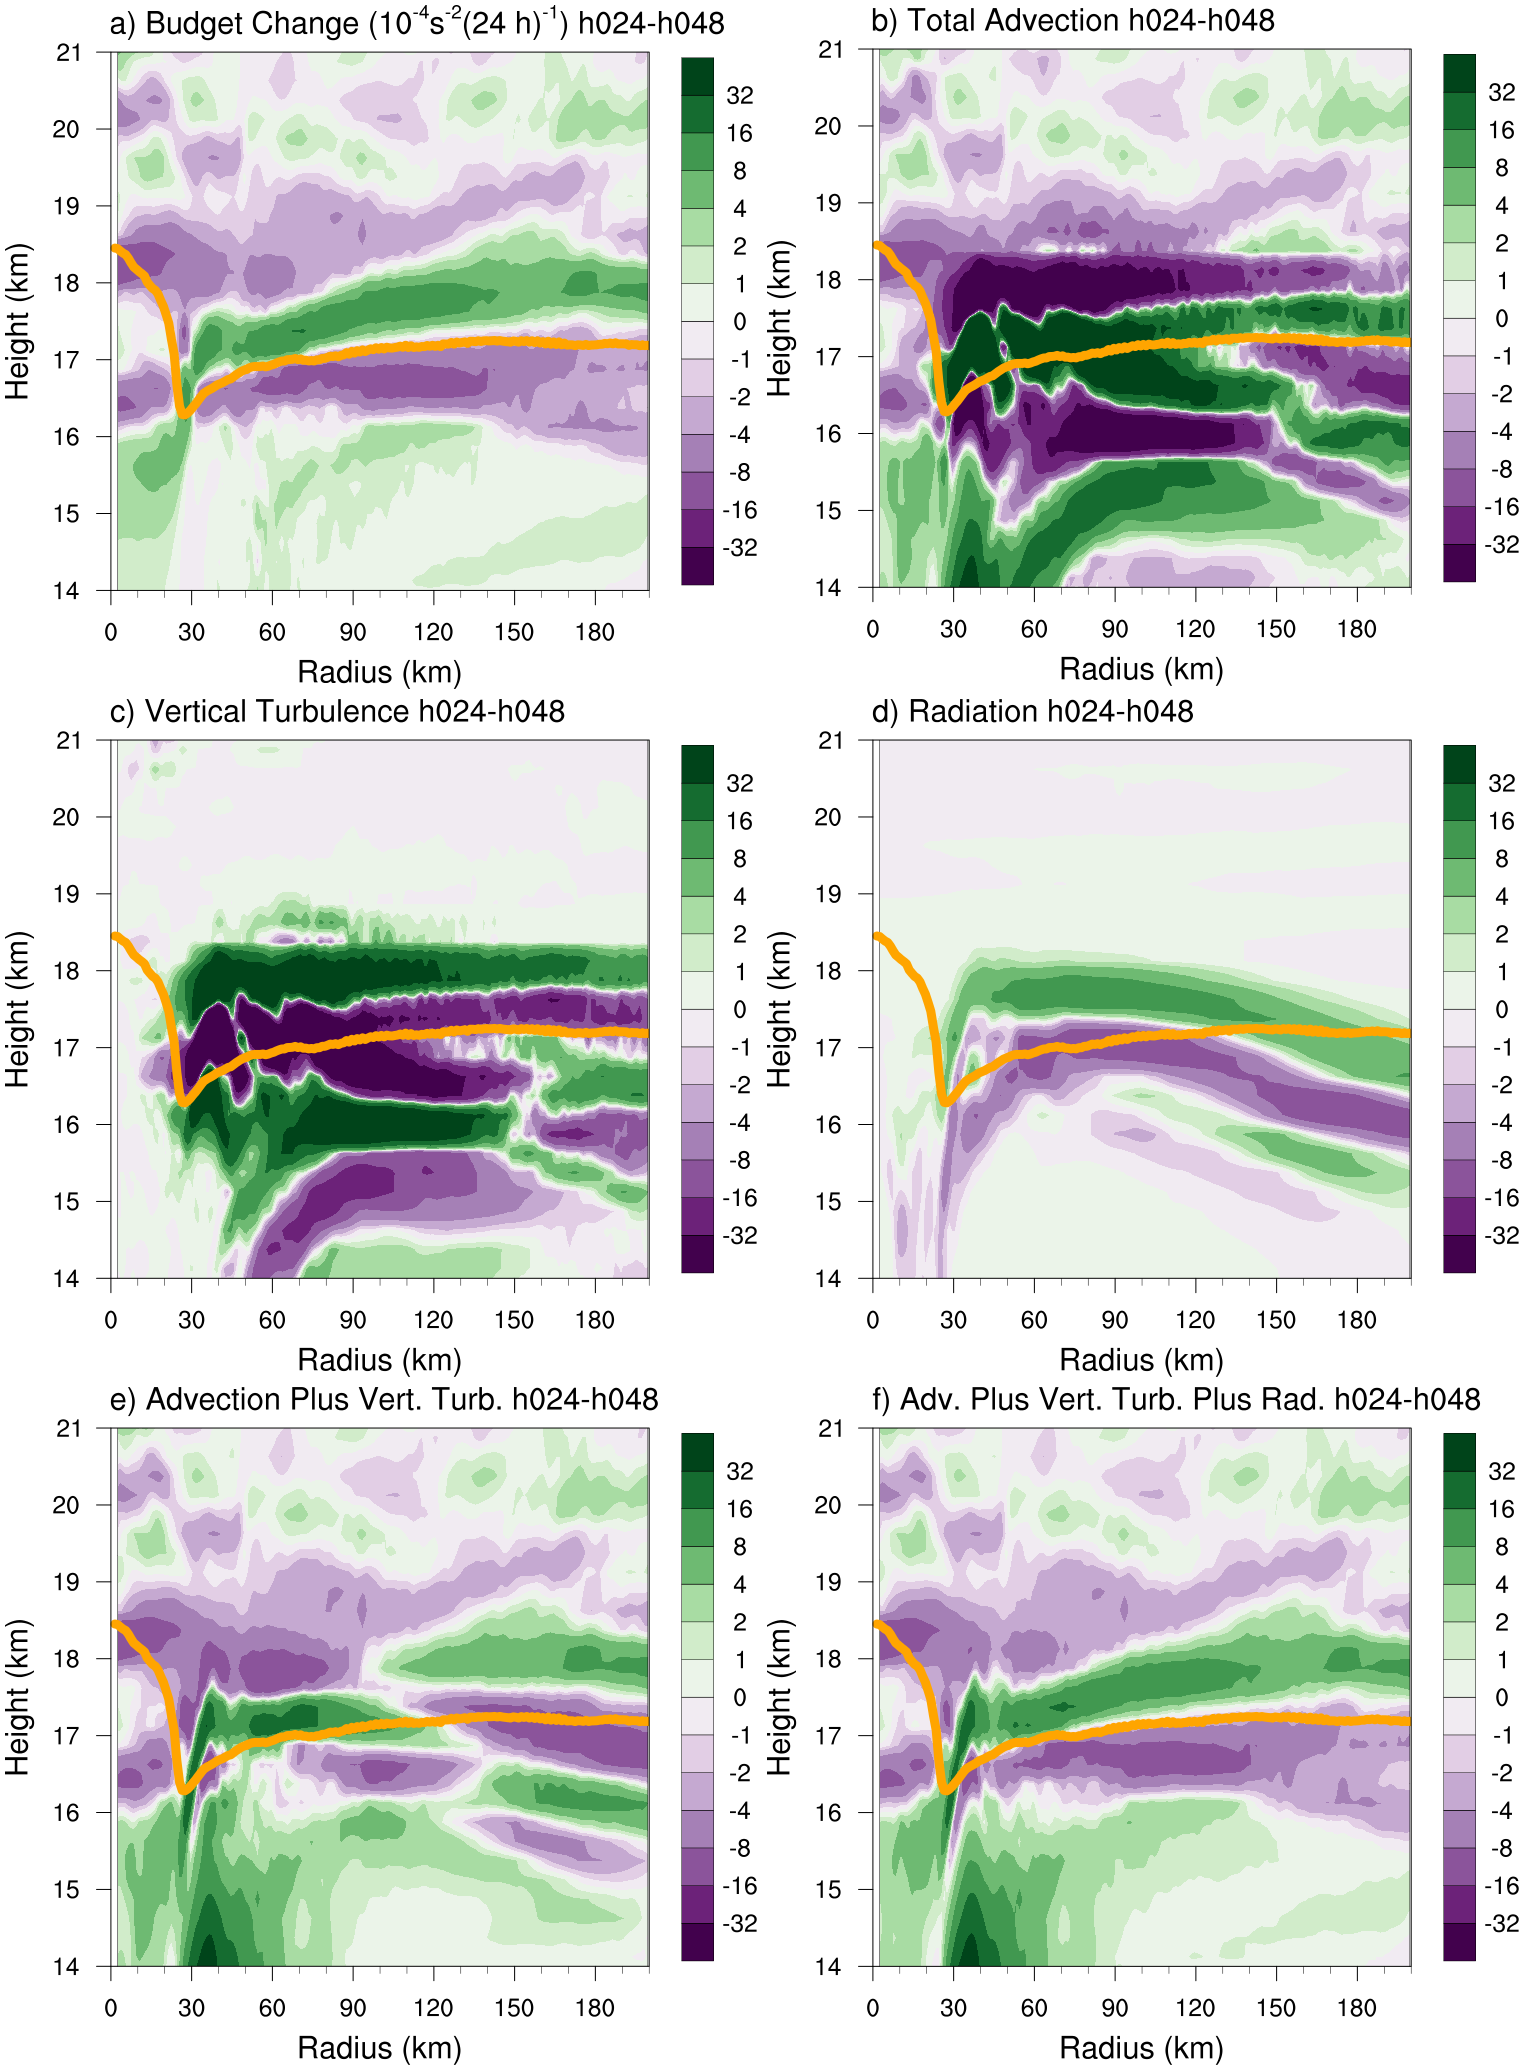
\includegraphics[width=27pc]{figures/h024-h048-budgetterms.png}}
\caption{As in Fig.~\ref{fig:stab-00-24}, but for the 24-48-hour period.}
\label{fig:stab-24-48}
\end{figure*}

%FIGURE 7%
\begin{figure*}[ht]
\centerline{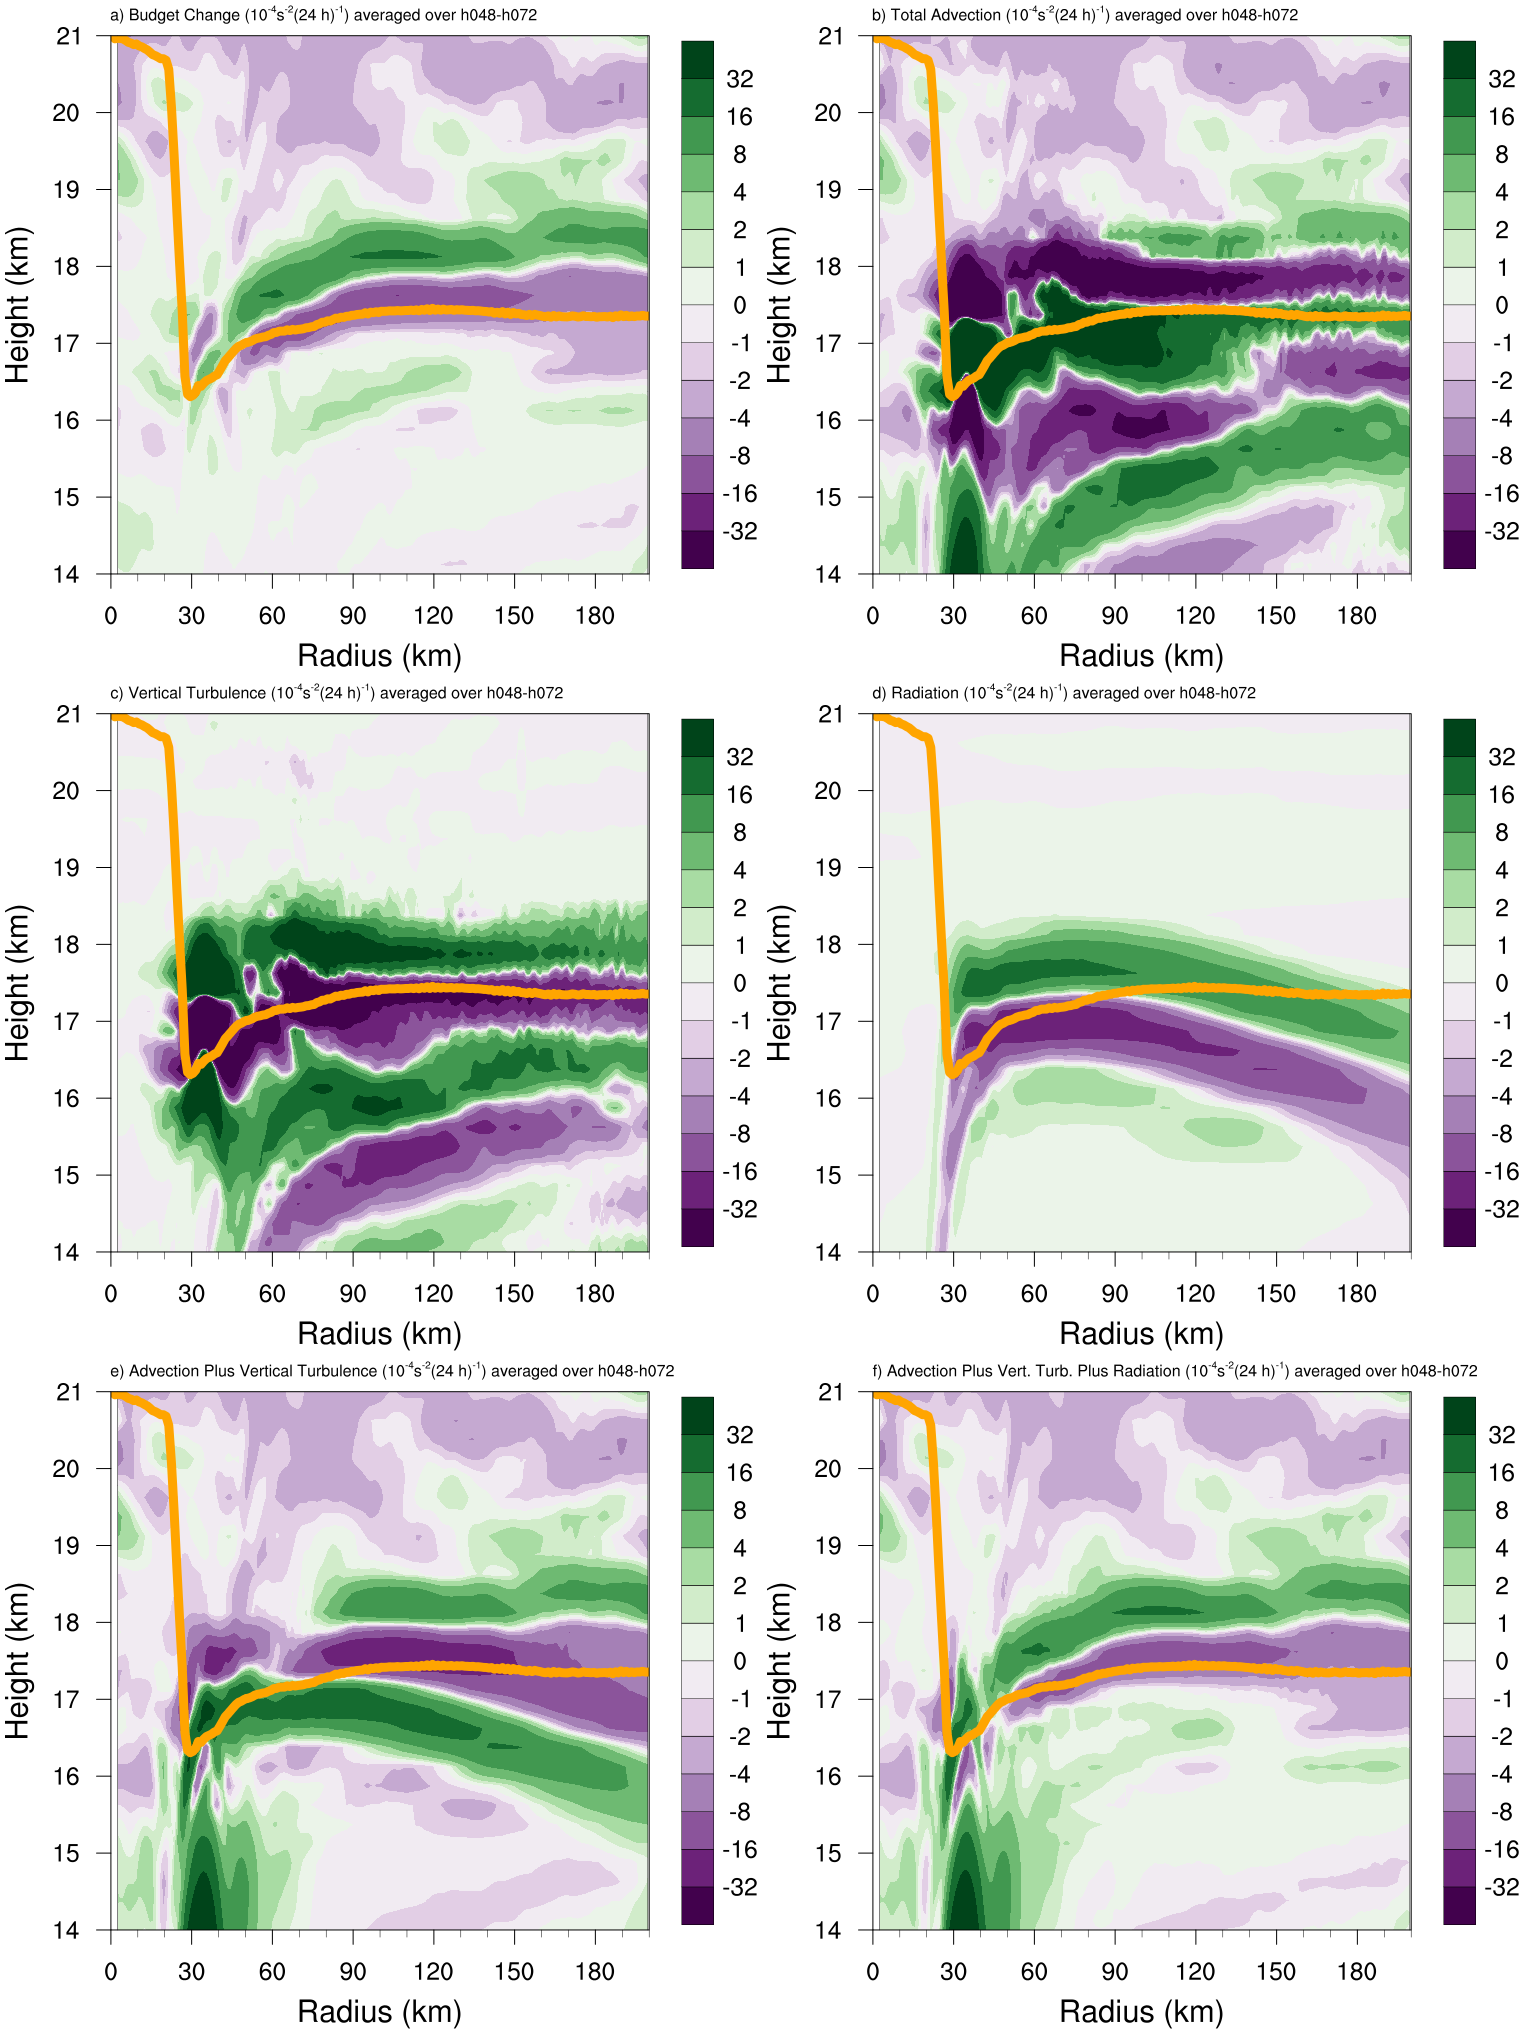
\includegraphics[width=27pc]{figures/h048-h072-budgetterms.png}}
\caption{As in Fig.~\ref{fig:stab-00-24}, but for the 48-72-hour period.}
\label{fig:stab-48-72}
\end{figure*}

%FIGURE 8%
%\begin{figure*}[ht]
%\centerline{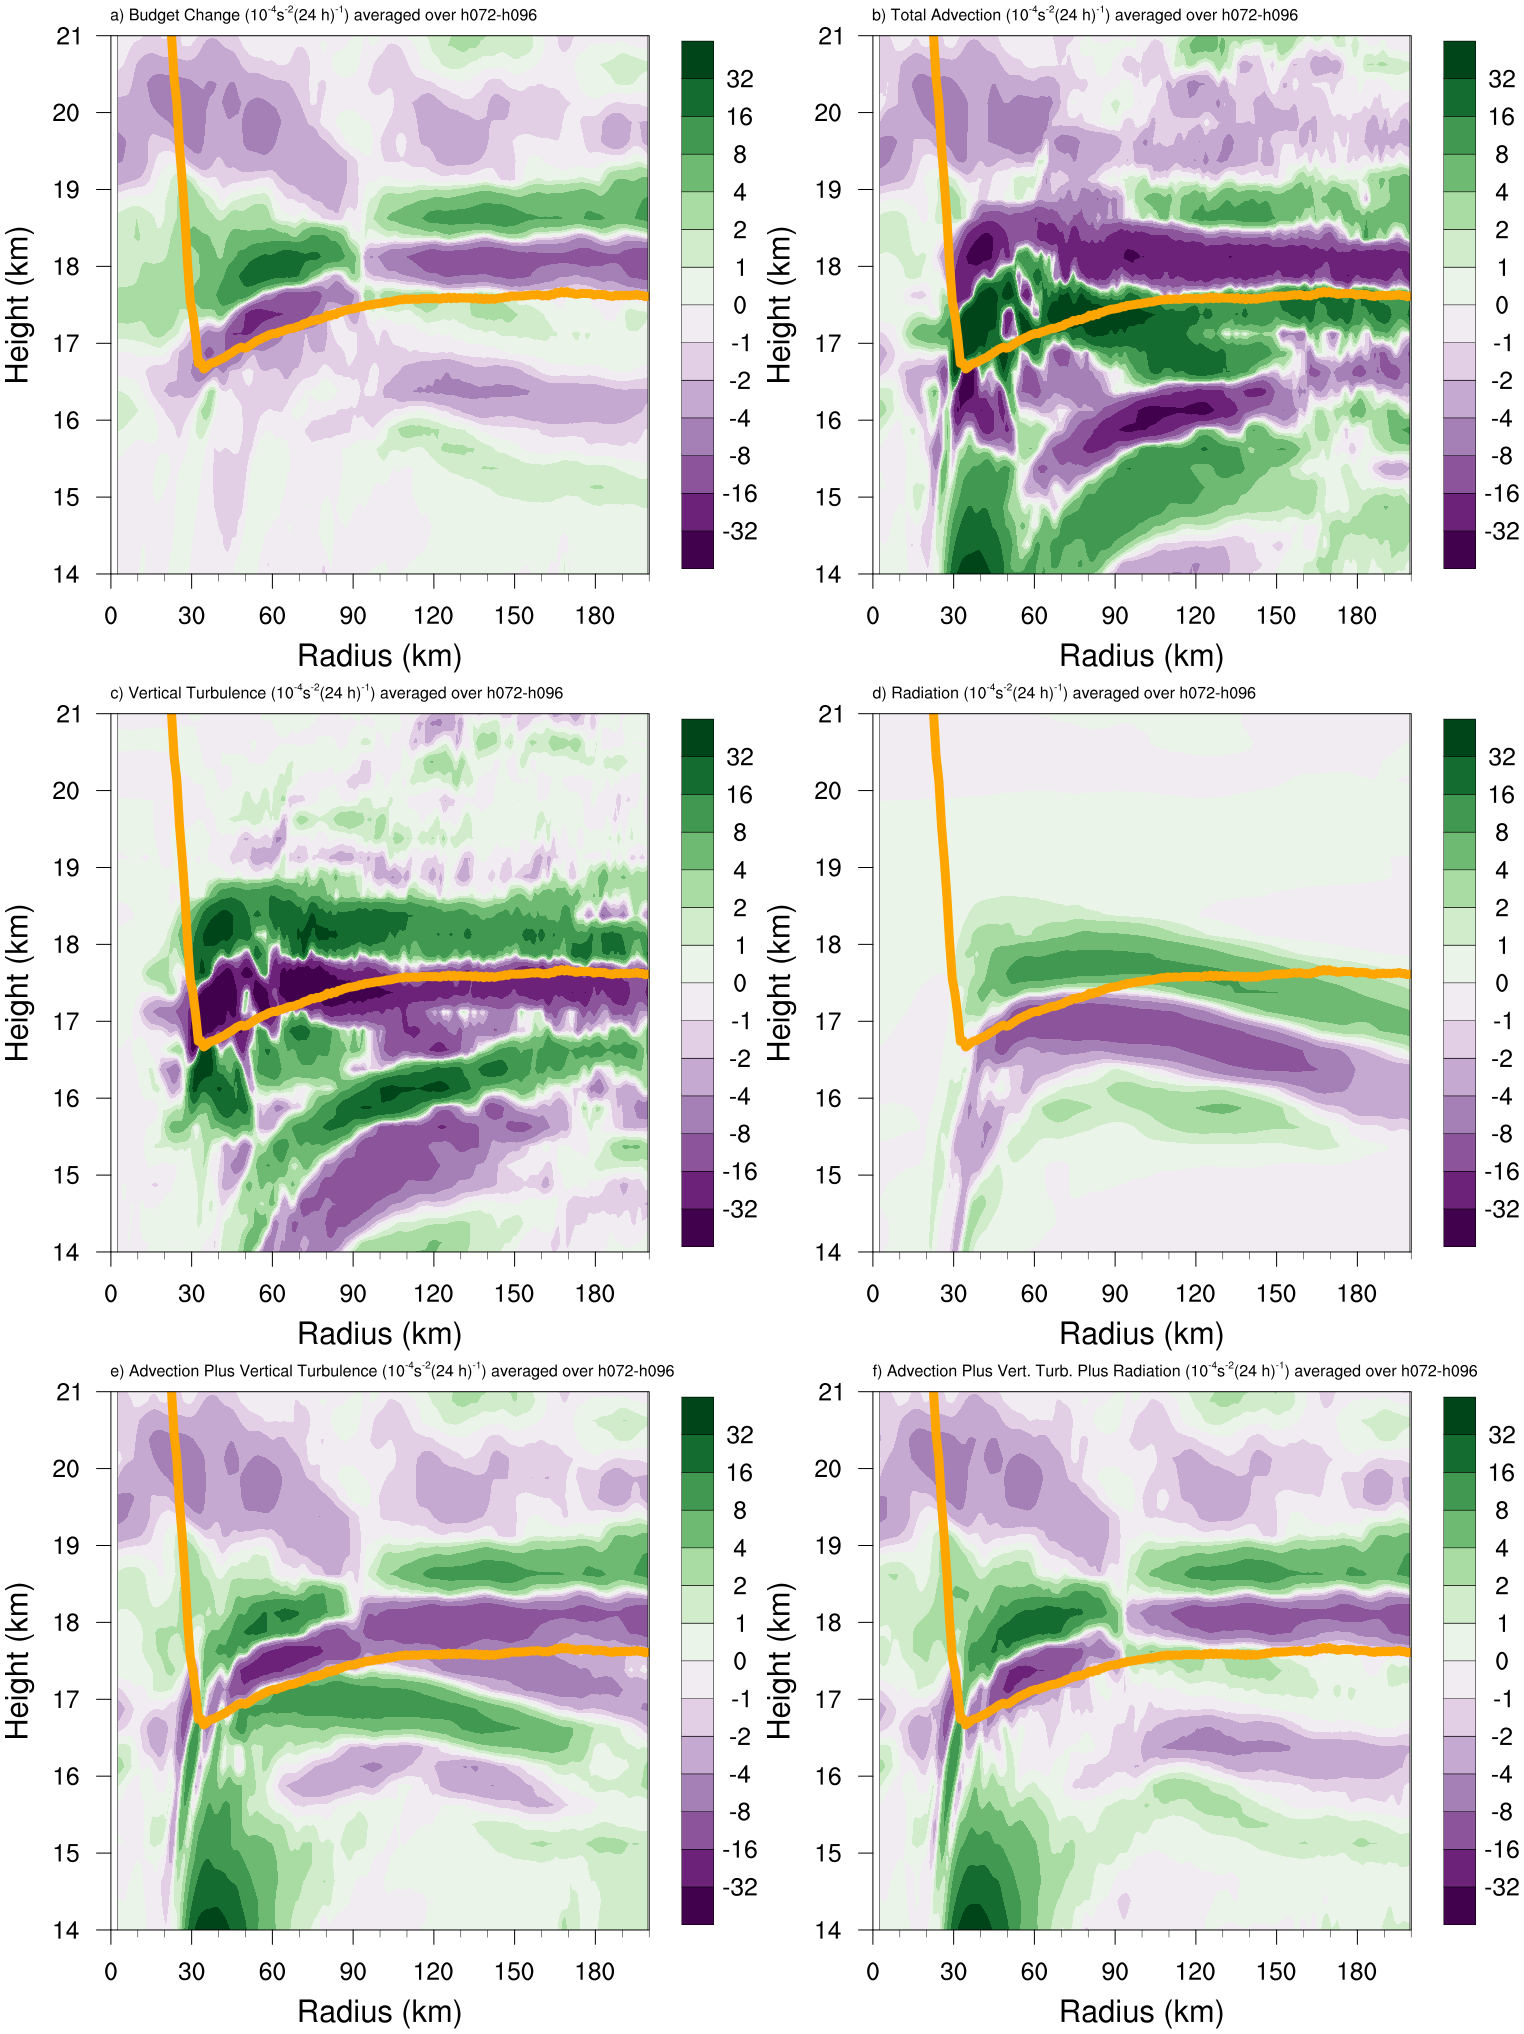
\includegraphics[width=33pc]{figures/h072-h096-budgetterms.png}}
%\caption{As in Fig.~\ref{fig:stab-48-72}, but for the 72-96-hour period.}
%\label{fig:stab-72-96}
%\end{figure*}

%FIGURE 8%
\begin{figure*}[ht]
\centerline{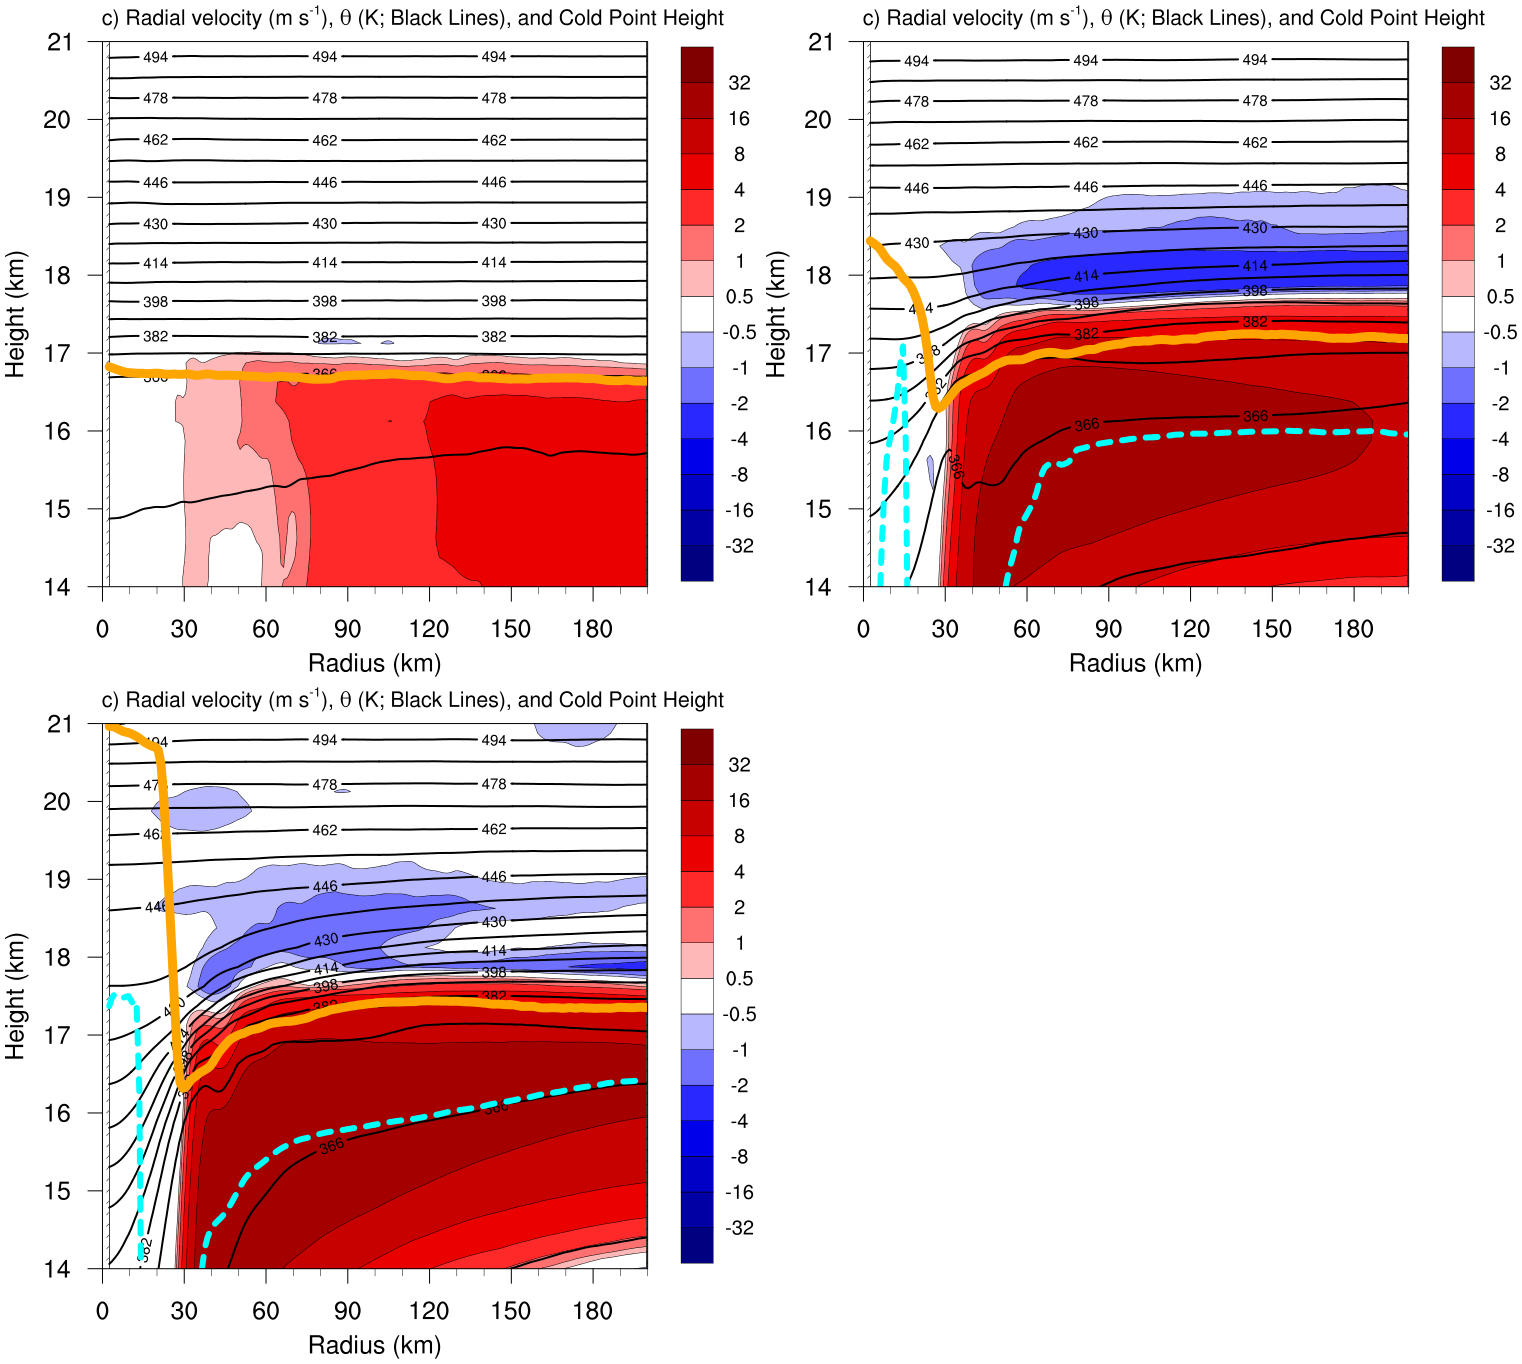
\includegraphics[width=39pc]{figures/u.png}}
\caption{Radial velocity (m s\textsuperscript{-1}; filled contours), potential temperature (K; thick black contours), and cold point tropopause height (orange lines) averaged over (a) 0-24 hours, (b) 24-48 hours, and (c) 48-72 hours.}
\label{fig:u}
\end{figure*}

%FIGURE 9%
\begin{figure*}[ht]
\centerline{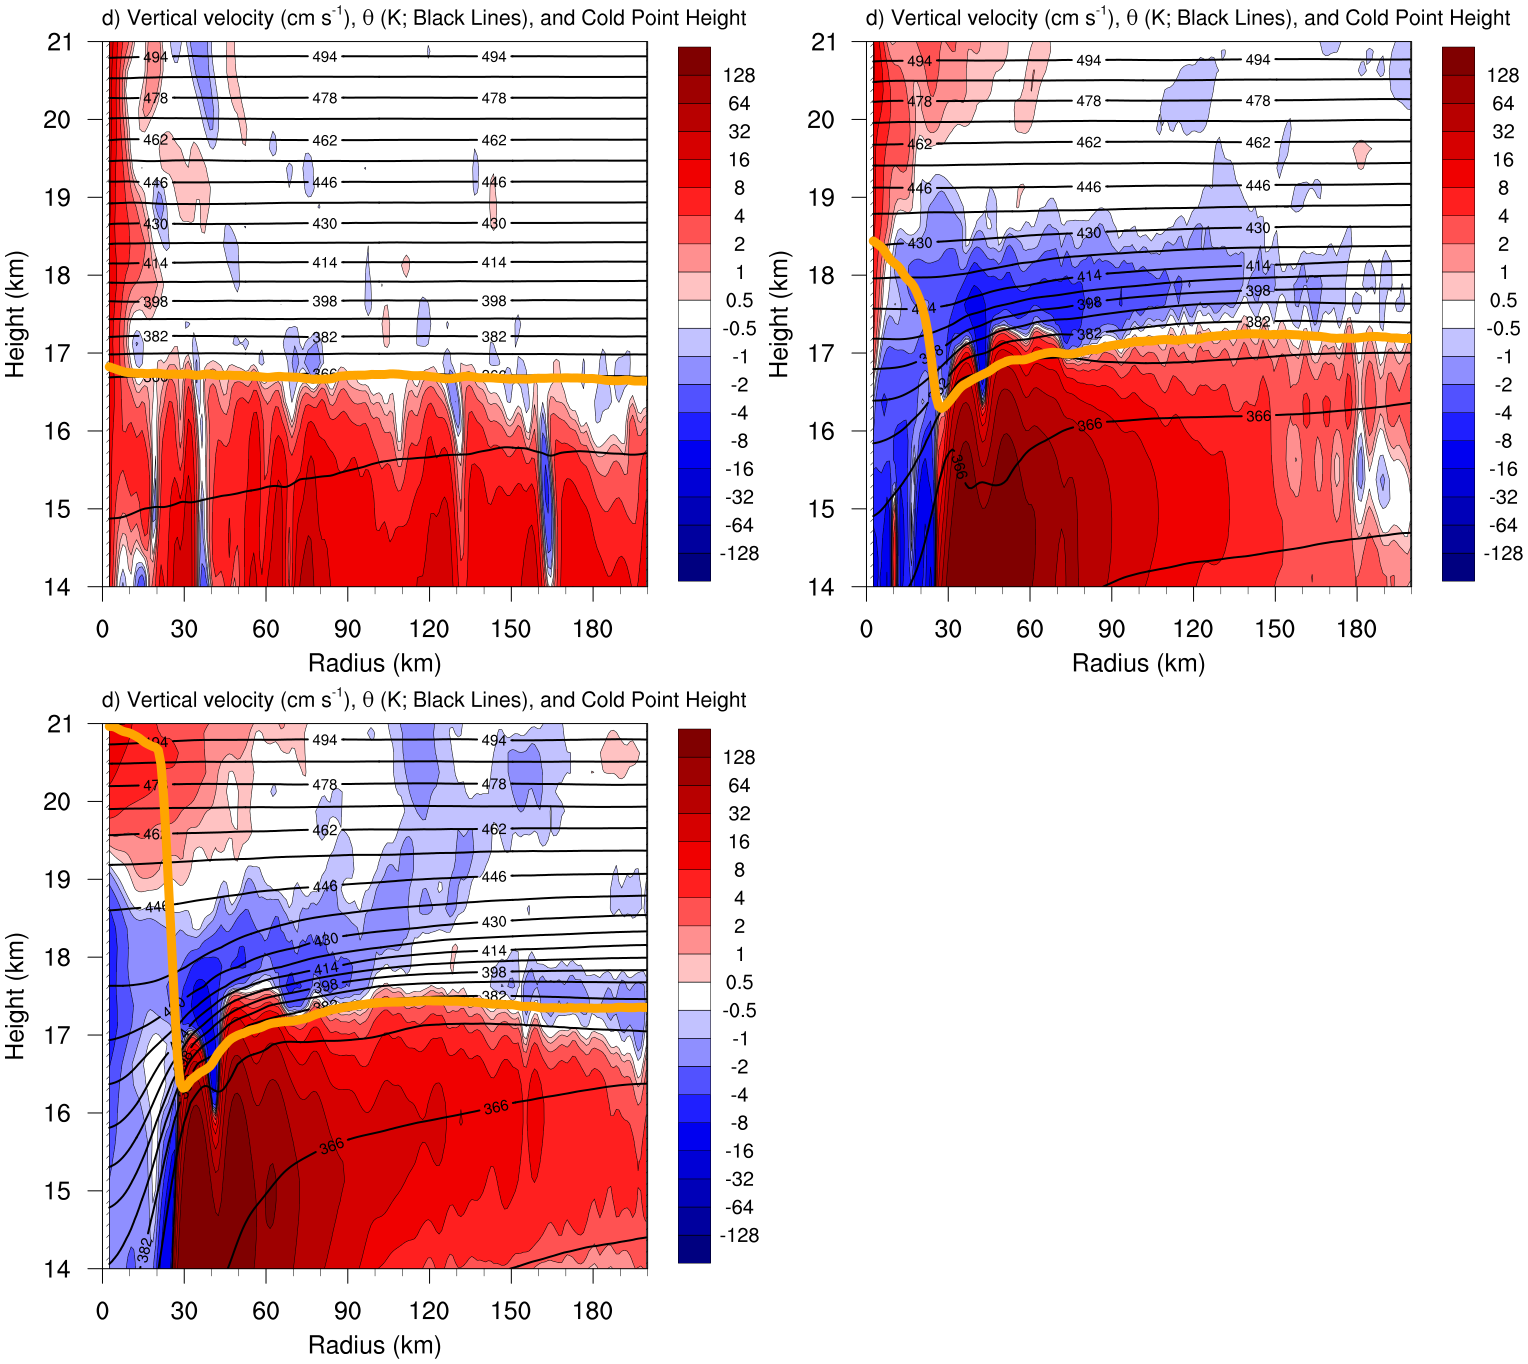
\includegraphics[width=39pc]{figures/w.png}}
\caption{Vertical velocity (cm s\textsuperscript{-1}; filled contours), potential temperature (K; thick black contours), and cold point tropopause height (orange lines) averaged over (a) 0-24 hours, (b) 24-48 hours, and (c) 48-72 hours.}
\label{fig:w}
\end{figure*}

%FIGURE 10%
\begin{figure*}[ht]
\centerline{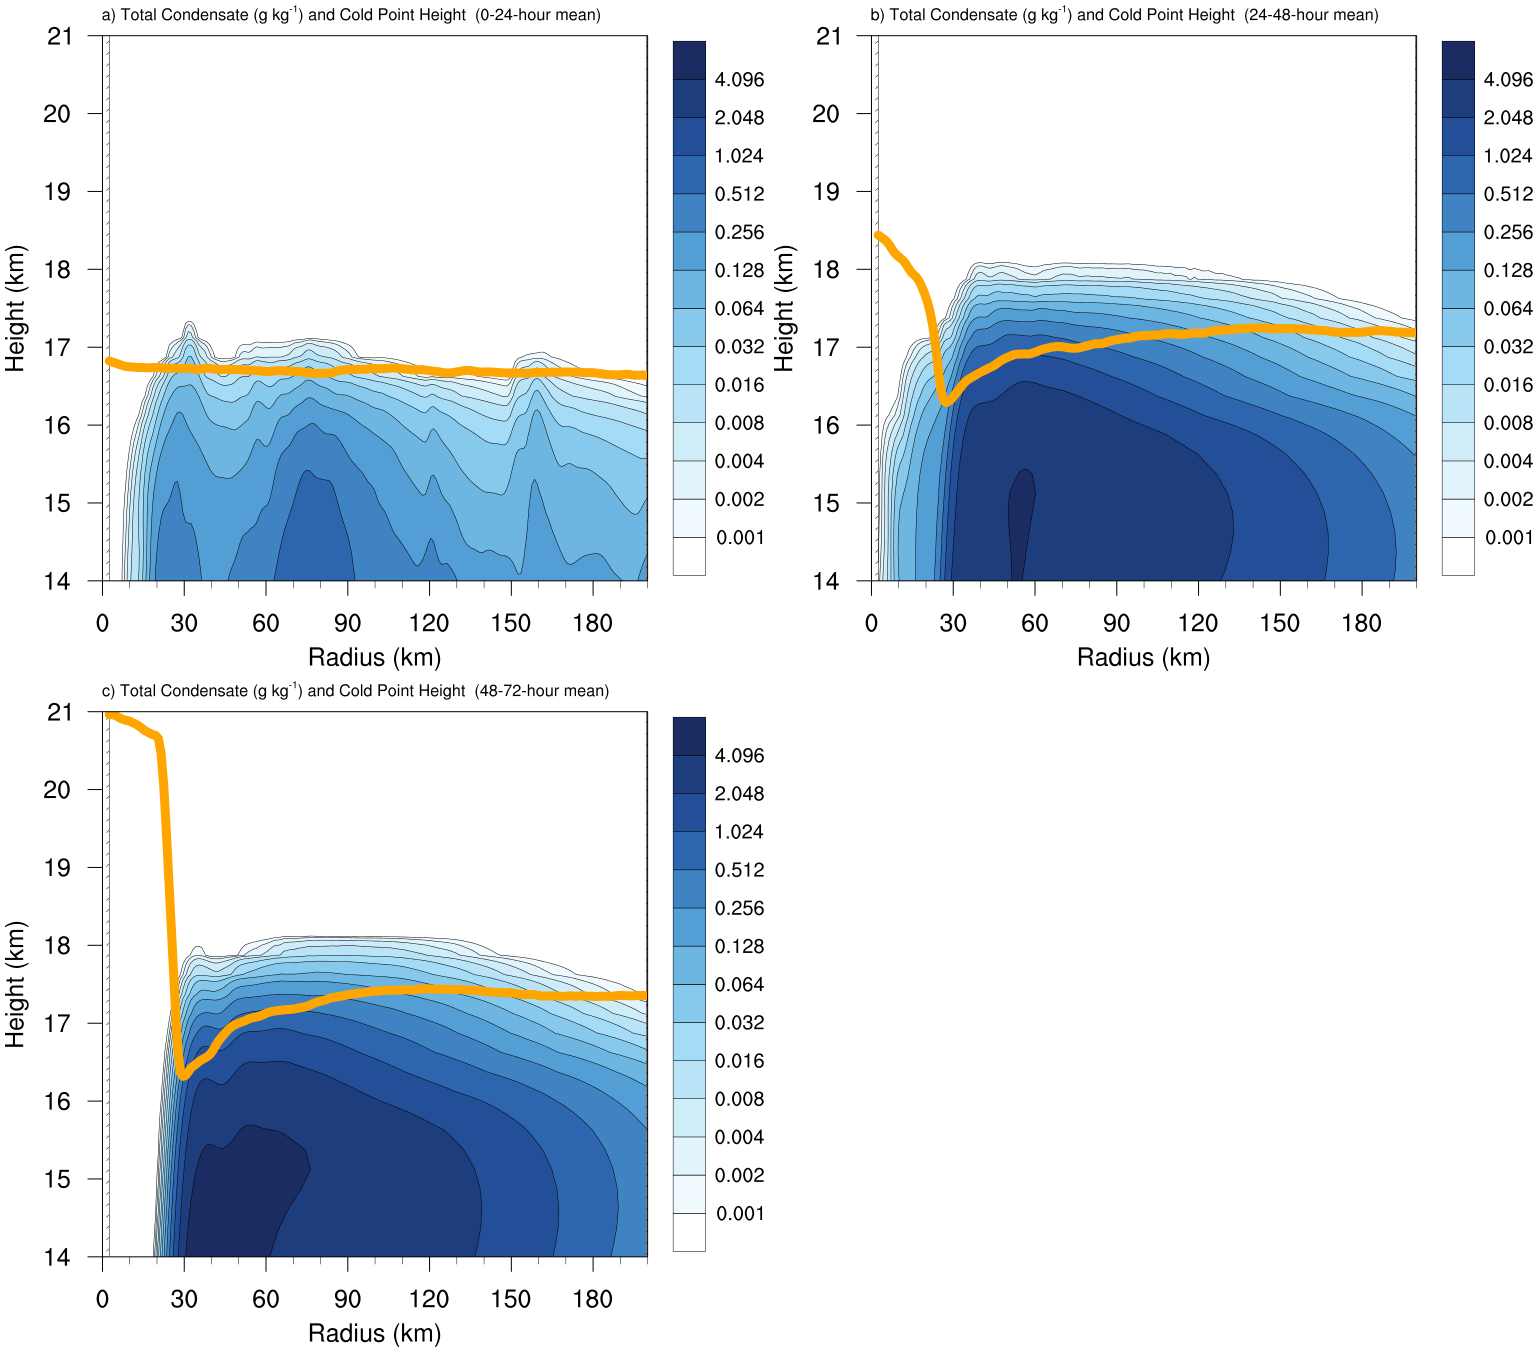
\includegraphics[width=39pc]{figures/qtot.png}}
\caption{Total condensate mixing ratio (g kg\textsuperscript{-1}) and cold point tropopause height (orange lines) averaged over (a) 0-24 hours, (b) 24-48 hours, and (c) 48-72 hours.}
\label{fig:qtot}
\end{figure*}

%FIGURE 11%
\begin{figure*}[ht]
\centerline{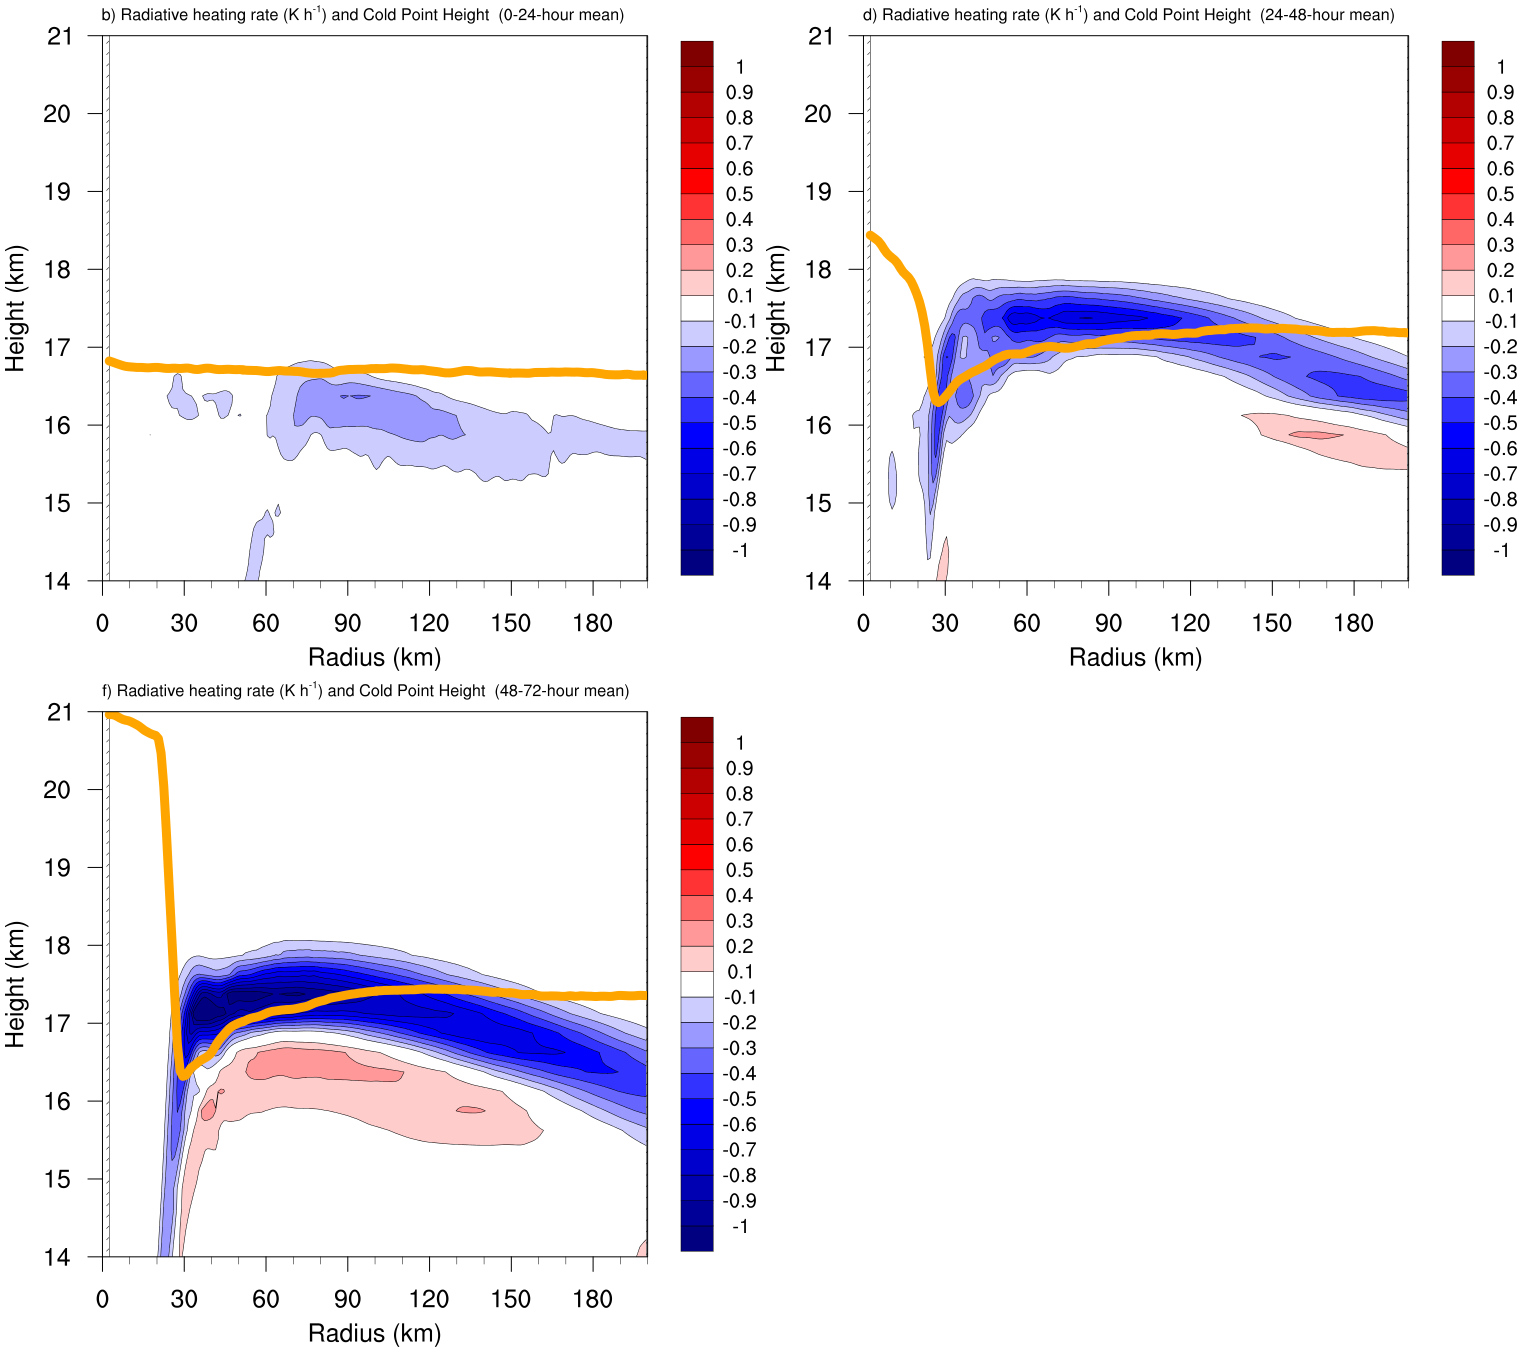
\includegraphics[width=39pc]{figures/radten.png}}
\caption{Radiative heating rate (K hr\textsuperscript{-1}) and cold point tropopause height (orange lines) averaged over (a) 0-24 hours, (b) 24-48 hours, and (c) 48-72 hours.}
\label{fig:radten}
\end{figure*}

%FIGURE 12%
\begin{figure*}[ht]
\centerline{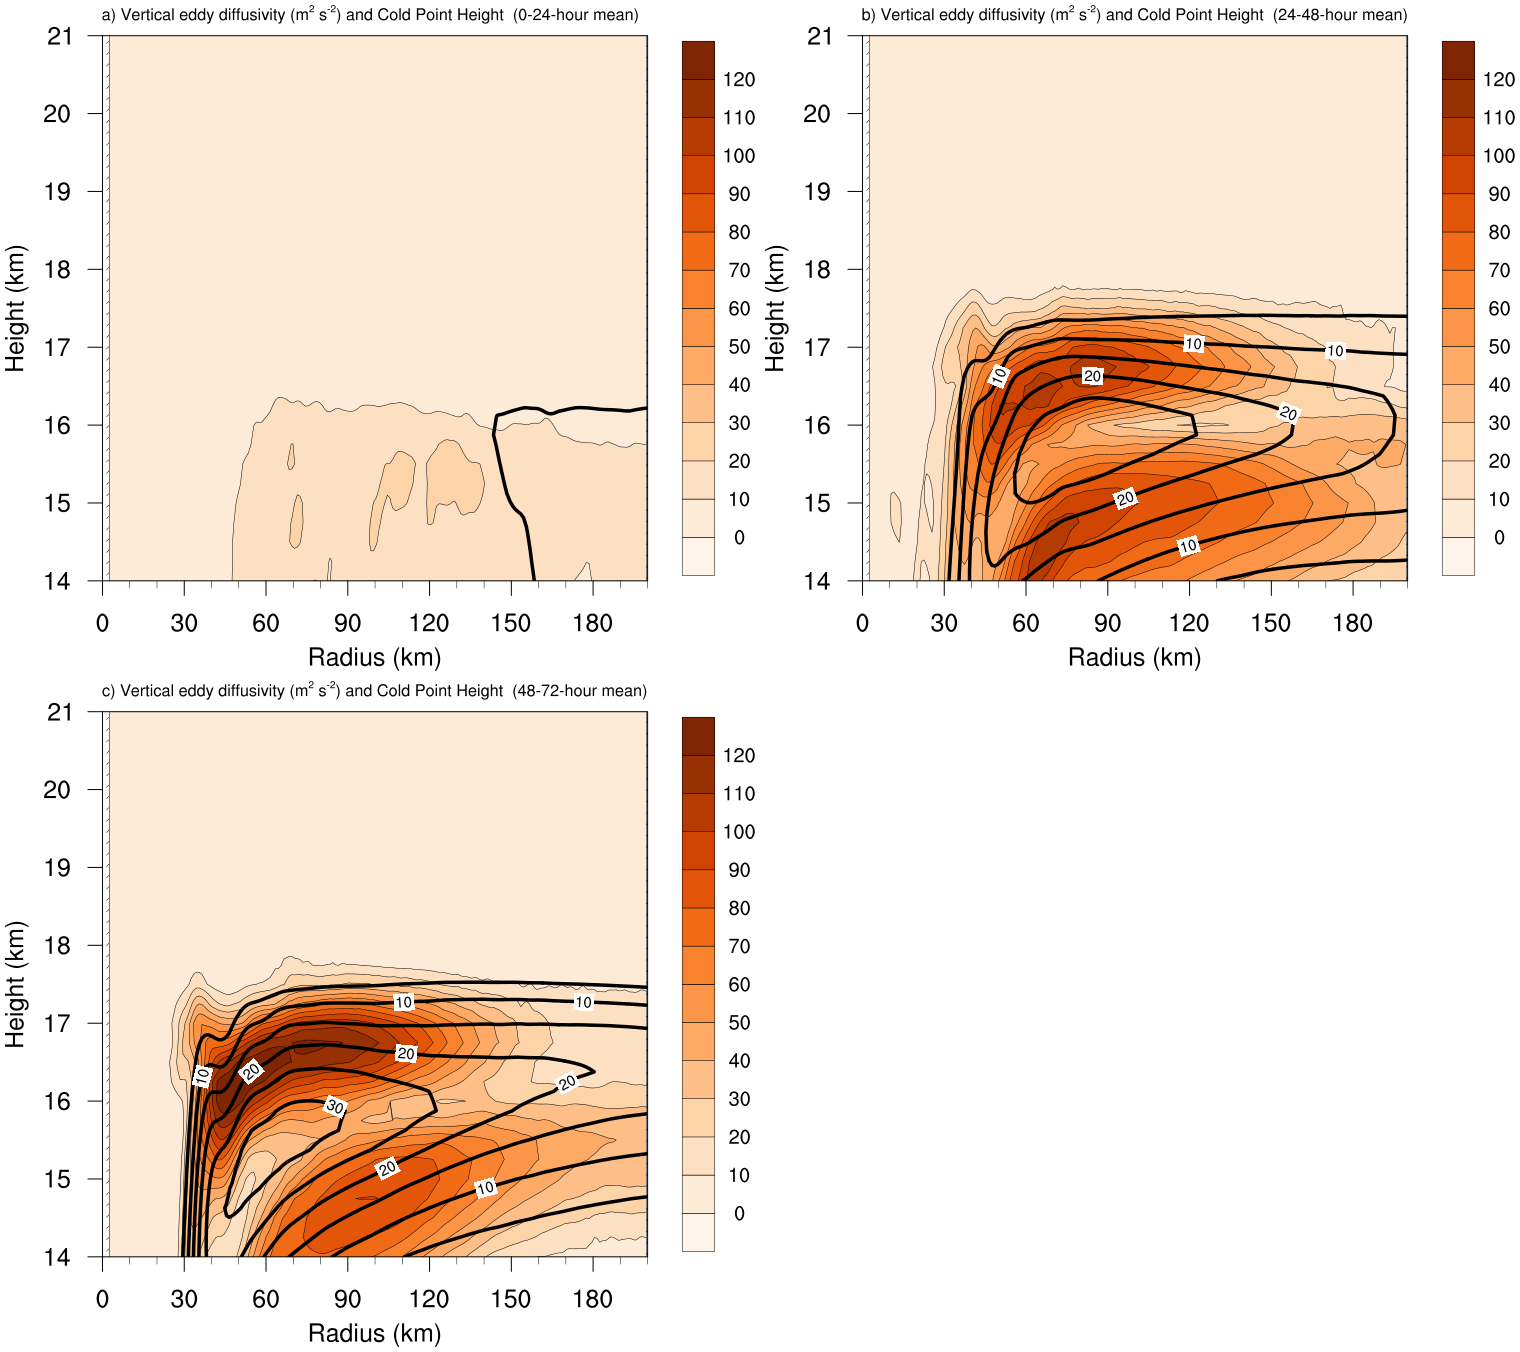
\includegraphics[width=39pc]{figures/khvten.png}}
\caption{Vertical eddy diffusivity (m\textsuperscript{2} s\textsuperscript{-2}; filled contours), cold point tropopause height (cyan lines), and radial velocity (m s\textsuperscript{-1}; thick black lines) averaged over (a) 0-24 hours, (b) 24-48 hours, and (c) 48-72 hours.}
\label{fig:radten}
\end{figure*}

%\begin{figure}[t]
%\begin{figure}[t]
%\begin{figure}[t]
%  \noindent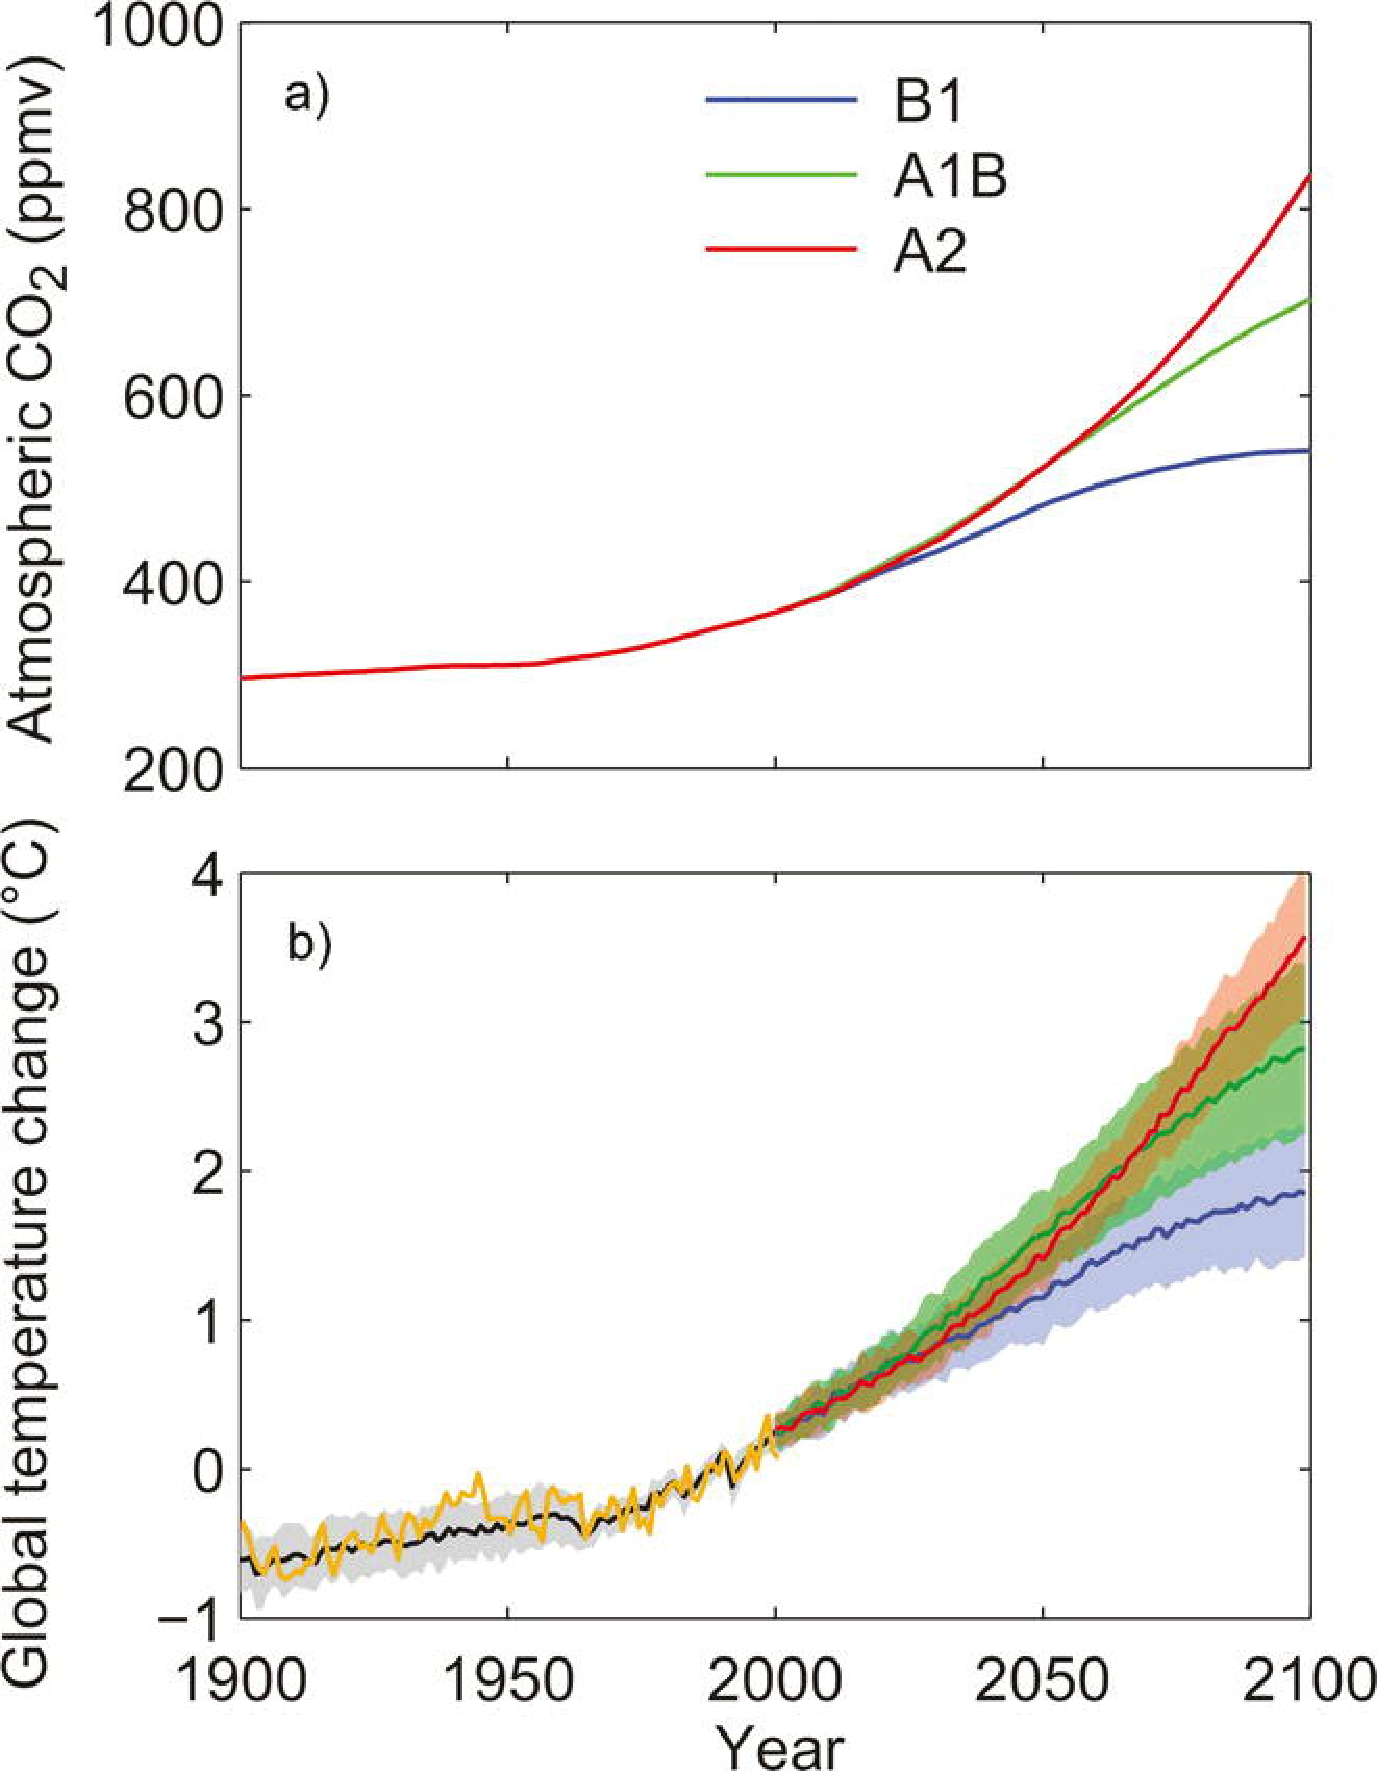
\includegraphics[width=19pc,angle=0]{figure01.pdf}\\
%  \caption{Enter the caption for your figure here.  Repeat as
%  necessary for each of your figures. Figure from \protect\cite{Knutti2008}.}\label{f1}
%\end{figure}

\end{document}
